\documentclass[draft]{agujournal2019}
\usepackage{url}
\usepackage{lineno}
\usepackage[inline]{trackchanges}
\usepackage{soul}
\usepackage{amsmath}
\usepackage{booktabs}
\usepackage{multirow}
% natbib compatibility aliases for apacite
\AtBeginDocument{%
  \let\citet\citeA
  \let\citep\cite
  \let\citealt\citeNP
  \let\citealp\citeNP
}
\linenumbers
\draftfalse

\journalname{JGR: Space Physics}

\begin{document}

\title{Predicting Ionospheric Cusp Location from Solar Wind: An XGBoost Model Trained on 27 Years of DMSP Data}

\authors{Yiwen~Zhu\affil{1}, Frank~R.~Toffoletto\affil{1}}

\affiliation{1}{Department of Physics and Astronomy, Rice University, Houston, TX, USA}

\correspondingauthor{F. Toffoletto}{toffo@rice.edu}

\begin{keypoints}
\item XGBoost predicts DMSP along-track equatorward cusp MLAT with MAE = 1.11\textdegree{} under temporal holdout (r = 0.886 on random splits), a 46\% MAE improvement over the best linear coupling function
\item The 60-minute mean Newell coupling function accounts for $\sim$31\% of gain-based feature importance, supporting the interpretation that cusp latitude responds to time-integrated reconnection over the preceding hour
\item Model skill degrades by 25\% during high auroral activity (AE $\geq$ 500~nT) but remains well below the linear baseline at all activity levels
\end{keypoints}

\begin{abstract}
The ionospheric cusp marks the narrow latitude band where magnetosheath plasma enters the magnetosphere along open field lines. Its equatorward boundary latitude shifts with the dayside reconnection rate, yet existing empirical models based on one or two coupling functions capture only a modest fraction of the crossing-to-crossing scatter ($r \approx 0.56$--$0.58$). We trained an XGBoost model on $\sim$40{,}000 Defense Meteorological Satellite Program (DMSP) cusp crossings spanning 1987--2014, using solar wind and interplanetary magnetic field (IMF) measurements together with their 15-, 30-, and 60-minute running statistics as inputs. The model predicts equatorward boundary latitude with a mean absolute error (MAE) of $\sim$1\textdegree{}, cutting the error of the \citet{newell2006cusp} linear baseline nearly in half. Leave-one-year-out cross-validation yields MAE = $1.26 \pm 0.19$\textdegree{} across 23 held-out years. Feature importance and partial dependence analyses show that the 60-minute mean Newell coupling function is the dominant predictor and that the model recovers established physical relationships, including the dipole tilt dependence and the nonlinear saturation of the coupling function. Because every input is available from upstream monitors at the Sun--Earth L1 point, the model is suitable for real-time cusp boundary forecasting.
\end{abstract}

\section*{Plain Language Summary}
Near the magnetic poles there is a narrow funnel---the cusp---through which solar wind plasma pours straight into the upper atmosphere. Its position shifts constantly, and getting that position wrong matters: GPS signals scintillate in the cusp, satellites experience extra drag, and polar-route aircrew face higher radiation doses. Until now the best predictions came from plugging one or two solar wind numbers into a simple formula, which explained only about half the crossing-to-crossing scatter. We approached this differently. We fed 27~years of DMSP satellite passes ($\sim$40{,}000 cusp crossings) into an XGBoost model together with 74 solar wind and IMF measurements---not just snapshots, but how each quantity changed over the preceding hour. The result: cusp latitude predicted to within $\sim$1\textdegree, cutting the error almost in half compared with earlier methods. What the model ``learned'' on its own agrees with decades of physics: cusp latitude tracks the reconnection rate integrated over roughly the past hour, not the solar wind you see right now. Because every input comes from upstream monitors already flying at L1, there is a clear path toward real-time cusp forecasting.

% ======================================================================
\section{Introduction}
\label{sec:intro}
% ======================================================================

\subsection{The Ionospheric Cusp and Its Importance}

The polar cusp is a narrow region on the dayside where the geomagnetic field allows magnetosheath plasma to enter the ionosphere directly \cite{pitout2021cluster}. At $\sim$840~km altitude, a DMSP pass through the cusp sees a $\sim$1--2\textdegree{} MLAT band of soft particle precipitation \cite{newell1988cusp}: ion energies below 3~keV, electron energies below 220~eV, and ion fluxes above $2 \times 10^7$~eV/(cm$^2$~s~sr~eV). The full cusp spans $\sim$3--4\textdegree{} MLAT and several hours of MLT \cite{zhang2013lfm, wing2005kp}. Its equatorward boundary shifts to lower latitudes when dayside reconnection is strong and moves back poleward when reconnection weakens \cite{newell2006cusp, newell2007coupling}.

Knowing where the cusp is matters in practice. GPS scintillation is enhanced in the cusp region due to ionospheric irregularities driven by soft precipitation and associated Joule heating \cite{pitout2021cluster}. Low-Earth-orbit satellites experience increased drag near the cusp due to thermospheric upwelling. The cusp is also relevant to radiation exposure of polar-route aviation and to the interpretation of ground-based radar and magnetometer data. Yet no operational model currently predicts cusp location from upstream solar wind data.

\subsection{Existing Cusp Location Models}

\citet{newell2006cusp} tested 10 coupling functions against DMSP cusp crossings from 1984--2005. The ``intermediate'' merging electric field $E_{WAV} = v B_T \sin^4(\theta_c/2)$ gave the best correlation: $r = 0.81$ on binned data, $r \approx 0.56$ on individual crossings. A nonlinear fit ($\Lambda_c = -3.65 \times 10^{-2} E_{WAV}^{2/3} + 77.2$\textdegree) pushed the binned correlation to $r = 0.83$. Their best results came from IMF data averaged over 60~minutes, pointing to the time-integrated reconnection rate rather than instantaneous values as the controlling quantity.

\citet{newell2007coupling} subsequently proposed the nearly universal coupling function $d\Phi_{MP}/dt = v^{4/3} B_T^{2/3} \sin^{8/3}(\theta_c/2)$, representing the rate of magnetic flux opening at the magnetopause. This function achieved $r = 0.845$ against $\sin(\Lambda_c)$ for cusp latitude (binned) and outperformed all other coupling functions across 10 different magnetospheric state variables.

\citet{newell1989tilt} established that dipole tilt angle shifts the cusp equatorward at a rate of approximately $-0.06$\textdegree/\textdegree{} of tilt. More recently, \citet{anderson2024cusp} used a 40-year, 41,000-crossing DMSP database to demonstrate that the tilt dependence varies with MLT sector and IMF $B_y$ sign, reflecting the asymmetric influence of $B_y$ on reconnection geometry \cite{cowley1981imfby}.

Global MHD simulations can reproduce cusp dynamics \cite{connor2015mhd, zhang2013lfm}, but a single run takes hours of CPU time---far too slow for real-time use. Every empirical model published so far relies on one or two solar wind parameters and a linear or low-order nonlinear fit.

\subsection{Machine Learning in Space Physics}

Machine learning has found growing use in space physics \citep{camporeale2019challenge, bortnik2021ml}. \citet{feng2025auroral} predicted auroral oval boundaries with XGBoost using Kp as input and found tree-based models outperformed neural networks. \citet{aghabozorgi2024magnetopause} applied ML to magnetopause standoff distance, with results limited mainly by OMNI propagation uncertainty. \citet{grinsztajn2022tree} showed more generally that tree-based models beat deep learning on tabular data---the kind of structured input we deal with here.

Cusp location prediction, however, has not yet been tackled with ML. Two properties of this problem favor tree-based methods. First, the cusp latitude depends on several solar wind parameters at once, and those dependencies are nonlinear---hard for a one- or two-parameter formula to represent. Second, what the solar wind did over the past hour matters as much as what it is doing now, because the magnetosphere takes roughly an hour to reconfigure after an IMF change.

\subsection{Present Study}

In this paper, we present the first machine learning prediction of cusp precipitation boundaries as observed along DMSP orbit tracks---specifically the equatorward and poleward MLAT and the equatorward and mean MLT of cusp-type ion precipitation at the MLT of each satellite crossing---from 74 solar wind and IMF features. These along-track boundaries are a one-dimensional snapshot of the cusp at a single MLT and differ from a complete two-dimensional cusp description, which would require either global simulations or simultaneous multi-point measurements. The equatorward boundary corresponds to the open--closed field line boundary at the crossing MLT and is the standard quantity in cusp latitude studies \citep{newell2006cusp, anderson2024cusp}. Our contributions are:

\begin{enumerate}
\item An XGBoost model achieving MAE = 1.11\textdegree{} under temporal holdout ($1.26 \pm 0.19$\textdegree{} under leave-one-year-out) for equatorward cusp MLAT ($r = 0.886$ on random splits), a 46\% improvement over the best linear coupling function on the same dataset.
\item Demonstration that 60-minute history features dominate prediction, which matches the expectation that cusp latitude tracks $\sim$1-hour integrated reconnection.
\item Gain-based feature importance, confirmed by SHAP, and partial dependence analysis recover known physical relationships and expose nonlinear interactions that single-coupling-function models miss.
\item Gradient-boosted trees outperform MLP, ResMLP, and TabTransformer on this tabular prediction problem.
\item All 74 inputs are derivable from upstream solar wind monitors, which means upstream solar wind data alone carry enough information to predict cusp boundary position with sub-degree accuracy.
\end{enumerate}

Section~\ref{sec:data} describes the data and methods; Section~\ref{sec:results} gives the results; Section~\ref{sec:discussion} discusses the physics and practical implications; Section~\ref{sec:conclusions} summarizes.

% ======================================================================
\section{Data and Methods}
\label{sec:data}
% ======================================================================

\subsection{DMSP Cusp Database}

We use cusp crossing identifications from the Defense Meteorological Satellite Program (DMSP) satellites F06 through F18, spanning 1987--2014 (27 years, approximately 2.5 solar cycles). The DMSP satellites fly in sun-synchronous polar orbits at $\sim$840~km altitude, carrying the SSJ/4 and SSJ/5 precipitating particle spectrometers \citep{hardy1984ssj4, redmon2017dmsp} that measure electron and ion differential energy fluxes from 30~eV to 30~keV across 19 logarithmically spaced energy channels.

Cusp crossings are identified using the criteria established by \citet{newell1988cusp}:
\begin{enumerate}
\item Average ion energy $\leq 3$~keV
\item Average electron energy $\leq 220$~eV
\item Total integral ion energy flux $\geq 2 \times 10^7$~eV/(cm$^2$~s~sr~eV)
\item Ion spectral flux peak between 100 and 7,000~eV
\end{enumerate}

For each crossing we record the equatorward and poleward boundary MLAT and MLT. These mark the along-track extent of cusp precipitation---a one-dimensional slice at the MLT of the satellite pass. The equatorward boundary approximates the open--closed field line boundary \cite{newell2006cusp, anderson2024cusp}, though DMSP precipitation-based identification can deviate from the true boundary far from noon or during complex reconnection geometries. Following \citet{anderson2024cusp}, we restrict the identification to 0830--1530~MLT to exclude skimming passes that cut the cusp at shallow angles and may produce unreliable poleward boundaries. Coordinates are Altitude-Adjusted Corrected Geomagnetic (AACGM-v2; \citealt{shepherd2014aacgm}). Of the 48,056 crossings in the raw database, 39,668 remain after removing records with missing solar wind data. About 90\% of crossings are in the Northern Hemisphere.

Figure~\ref{fig:data_coverage} shows the temporal (panel a, color-coded by satellite) and spatial (panels b--c, MLAT-MLT polar plots for each hemisphere) distribution of the dataset.

\begin{figure}[htbp]
\centering
\noindent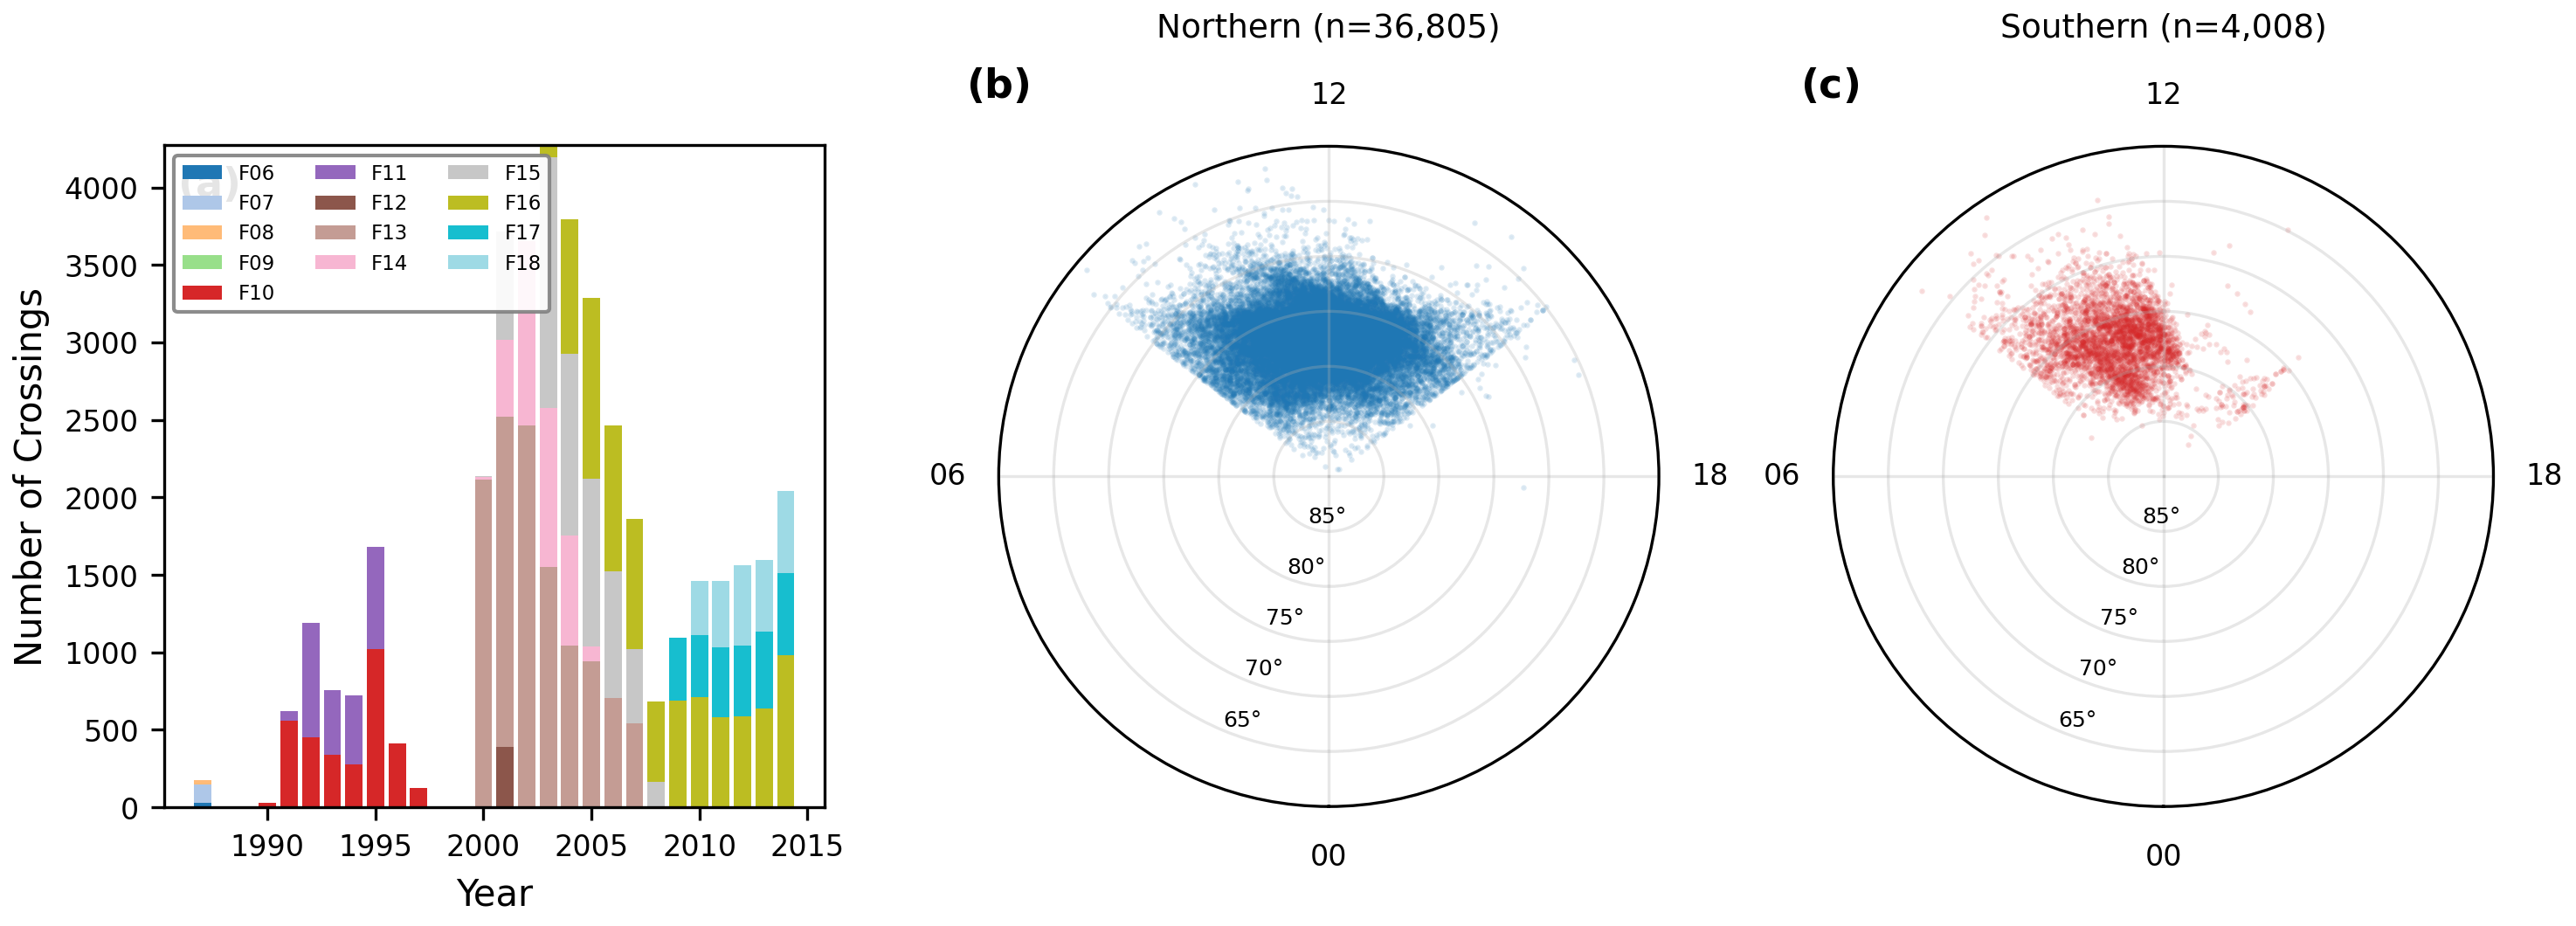
\includegraphics[width=0.9\textwidth]{figures/fig01_data_coverage.png}
\caption{Dataset overview. (a) Number of cusp crossings per year, color-coded by DMSP satellite (F06--F18). (b) Northern Hemisphere crossing locations ($n = 36{,}805$) and (c) Southern Hemisphere crossing locations ($n = 4{,}008$) in MLAT-MLT polar coordinates.}
\label{fig:data_coverage}
\end{figure}

\subsection{Solar Wind and IMF Features}

Solar wind and IMF parameters are obtained from the OMNI dataset \cite{king2005omni}, which provides time-shifted measurements propagated to the bow shock nose. For each cusp crossing, we extract the following categories of features:

\textbf{Base parameters (16 features):} Dipole tilt angle, hemisphere code (N/S), day of year, IMF components ($B_x$, $B_y$, $B_z$), solar wind bulk velocity ($v$), proton density ($n$), dynamic pressure ($P_{dyn}$), transverse IMF magnitude ($B_T = \sqrt{B_y^2 + B_z^2}$), IMF clock angle ($\theta_c = \text{atan2}(B_y, B_z)$, quadrant-aware), $\sin(\theta_c/2)$, Newell coupling function ($d\Phi_{MP}/dt = v^{4/3} B_T^{2/3} |\sin(\theta_c/2)|^{8/3}$; \citet{newell2007coupling}), Kan-Lee merging electric field ($E_{KL} = v B_T \sin^2(\theta_c/2)$; \citet{kan1979reconnection}), half-wave rectified $vB_s$ ($= v \max(-B_z, 0)$), and hemisphere-adjusted $B_y$ ($= B_y \times \text{sign}(\text{hemisphere})$).

\textbf{History features (58 features):} For each of six base parameters ($B_x$, $B_y$, $B_z$, $v$, $n$, $P_{dyn}$) we take the mean, standard deviation, and change ($\Delta$) over the preceding 15, 30, and 60~minutes---54 features in all. Four more come from the 60-minute mean and time-integral of $d\Phi_{MP}/dt$ and $vB_s$. Table~\ref{tab:features} lists the complete 74-feature set.

\begin{table}[htbp]
\centering
\caption{Summary of the 74 input features grouped by category.}
\label{tab:features}
\begin{tabular}{lll}
\toprule
Category & Count & Features \\
\midrule
Geometry & 3 & dipole\_tilt, hemi\_code, day\_of\_year \\
Raw IMF & 3 & $B_x$, $B_y$, $B_z$ \\
Solar wind & 3 & $v$, $n$, $P_{dyn}$ \\
Derived coupling & 7 & $B_T$, $\theta_c$, $\sin(\theta_c/2)$, $d\Phi_{MP}/dt$, $E_{KL}$, $vB_s$, $B_y \cdot \text{sgn}(\text{hemi})$ \\
15-min history & 18 & mean, std, $\Delta$ for $B_x$, $B_y$, $B_z$, $v$, $n$, $P_{dyn}$ \\
30-min history & 18 & mean, std, $\Delta$ for $B_x$, $B_y$, $B_z$, $v$, $n$, $P_{dyn}$ \\
60-min history & 22 & mean, std, $\Delta$ for $B_x$, $B_y$, $B_z$, $v$, $n$, $P_{dyn}$; \\
& & mean and integral of $d\Phi_{MP}/dt$ and $vB_s$ \\
\midrule
\textbf{Total} & \textbf{74} & \\
\bottomrule
\end{tabular}
\end{table}

\subsection{XGBoost Model}

We employ XGBoost (eXtreme Gradient Boosting; \citet{chen2016xgboost}), a gradient-boosted decision tree algorithm that builds an ensemble of regression trees sequentially, where each new tree fits the residual errors of the preceding ensemble. At each boosting round, XGBoost selects the tree structure (split features and thresholds) that maximizes the reduction in a regularized objective function combining the squared-error loss with L1 and L2 penalties on the leaf weights, discouraging overly complex trees. The final prediction is the sum of contributions from all trees. Because the ensemble is additive and each tree can split on any feature, XGBoost captures nonlinear relationships and multi-way interactions without the user having to specify a functional form. This is the central difference from the fixed-form coupling functions used in prior cusp studies.

We use scikit-learn's \texttt{MultiOutputRegressor} wrapper, which trains one independent XGBoost model per target variable, to predict the four targets separately: $|\text{eq\_MLAT}|$, $|\text{pole\_MLAT}|$, eq\_MLT, and mean\_MLT. We use absolute MLAT values to combine both hemispheres, with the hemisphere code included as an input feature to capture N/S asymmetries.

The hyperparameters were selected via systematic grid search over a development set: 1,000 boosting rounds, maximum tree depth of 8, learning rate of 0.02, row subsampling ratio of 0.8, column subsampling ratio of 0.7, L1 regularization $\alpha = 0.1$, L2 regularization $\lambda = 1.0$, and minimum child weight of 5. The relatively conservative learning rate and regularization parameters were chosen to mitigate overfitting, following the recommendations of \citet{lockwood2022pitfalls} regarding the risks of overparameterized coupling function fitting.

\subsection{Model Evaluation}

The dataset is split into 80\% training and 20\% test sets using a fixed random seed (42). Because DMSP crossings within the same day or storm interval are not independent, this random split likely provides optimistic performance estimates. We therefore treat the temporal holdout (train pre-2008, test 2008--2014) and leave-one-year-out (LOYO) cross-validation as primary performance metrics for assessing real-world generalization, and report the random-split metrics for comparison with prior single-crossing studies. We evaluate model performance using:

\begin{itemize}
\item Mean Absolute Error (MAE)
\item Root Mean Square Error (RMSE)
\item Coefficient of determination ($R^2$)
\item Pearson correlation coefficient ($r$)
\item Percentage of predictions within 1\textdegree, 2\textdegree, and 3\textdegree{} of observed values
\end{itemize}

We compare against a structured baseline ladder designed to isolate the sources of improvement:
\begin{enumerate}
\item \textit{Physics-motivated single-predictor fits}: linear regression on $B_z$, $vB_s$, $E_{KL}$, and $d\Phi_{MP}/dt$, and the nonlinear Newell baseline ($\Lambda_c = a \, E_{WAV}^{2/3} + b$, fitted via least squares; \citealt{newell2006cusp}). These represent the state of the art prior to this work.
\item \textit{Ridge regression on all 74 features} ($\ell_2$-regularized linear regression, $\alpha = 1.0$, features standardized): directly isolates gains attributable to feature richness from those attributable to the nonlinear model class, since both use the same inputs.
\item \textit{Gradient Boosting Regressor} (GBR, 300 trees, depth 5): a standard gradient-boosted tree baseline isolating the effect of nonlinear modeling from XGBoost's extended hyperparameter tuning (1,000 rounds, deeper trees).
\item \textit{Neural network architectures}: MLP, ResMLP, and TabTransformer, all trained on the same data splits with hyperparameter search via the same development set.
\end{enumerate}
This ladder allows us to attribute performance gains to: (a) richer predictor set, (b) nonlinear modeling, and (c) architectural differences within the tree vs.\ neural-network classes.

\subsection{Interpretability Methods}

To ensure physical interpretability, we employ two primary methods: (1) XGBoost's built-in gain-based feature importance, which quantifies each feature's contribution to reducing the loss function across all trees; and (2) partial dependence plots, which show the marginal effect of each feature on the prediction, averaged over all other features. As a cross-check on the gain ranking, we also compute SHAP (SHapley Additive exPlanations; \citealt{lundberg2017shap}) values on a subset of test-set samples; SHAP provides theoretically grounded, per-prediction feature attributions based on cooperative game theory. Because several features are strongly correlated (e.g., $vB_s$ and $d\Phi_{MP}/dt$), importance and partial dependence values reflect marginal rather than causal contributions and should be read accordingly.

% ======================================================================
\section{Results}
\label{sec:results}
% ======================================================================

\subsection{Model Performance and Comparison With Baselines}

Table~\ref{tab:performance} summarizes the XGBoost model's performance on the held-out test set for all four prediction targets. The equatorward boundary latitude is predicted with MAE = 0.97\textdegree{} and $r = 0.886$, while the poleward boundary achieves MAE = 0.95\textdegree{} and similar correlation. MLT predictions achieve MAE values of 0.77~hr (eq\_MLT) and 0.73~hr (mean\_MLT), with lower $R^2$ values (0.48 and 0.51) because the cusp's MLT distribution is intrinsically narrow. Scatter plots of predicted versus observed values appear in Figure~\ref{fig:scatter}, with color encoding point density. For both MLAT targets (panels a, b), points cluster tightly around the 1:1 line over the full 62--82\textdegree{} range. The MLT panels (c, d) bunch near 12~MLT, as one would expect from the cusp's noon-sector concentration.

\begin{table}[htbp]
\centering
\caption{XGBoost model performance on the test set for all four cusp boundary parameters.}
\label{tab:performance}
\begin{tabular}{lcccc}
\toprule
Target & MAE & RMSE & $R^2$ & $r$ \\
\midrule
$|$eq MLAT$|$ (\textdegree) & 0.97 & 1.34 & 0.79 & 0.887 \\
$|$pole MLAT$|$ (\textdegree) & 0.95 & 1.31 & 0.79 & 0.888 \\
eq MLT (hr) & 0.77 & 1.01 & 0.48 & 0.700 \\
mean MLT (hr) & 0.73 & 0.98 & 0.49 & 0.709 \\
\bottomrule
\end{tabular}
\end{table}

\begin{figure}[htbp]
\centering
\noindent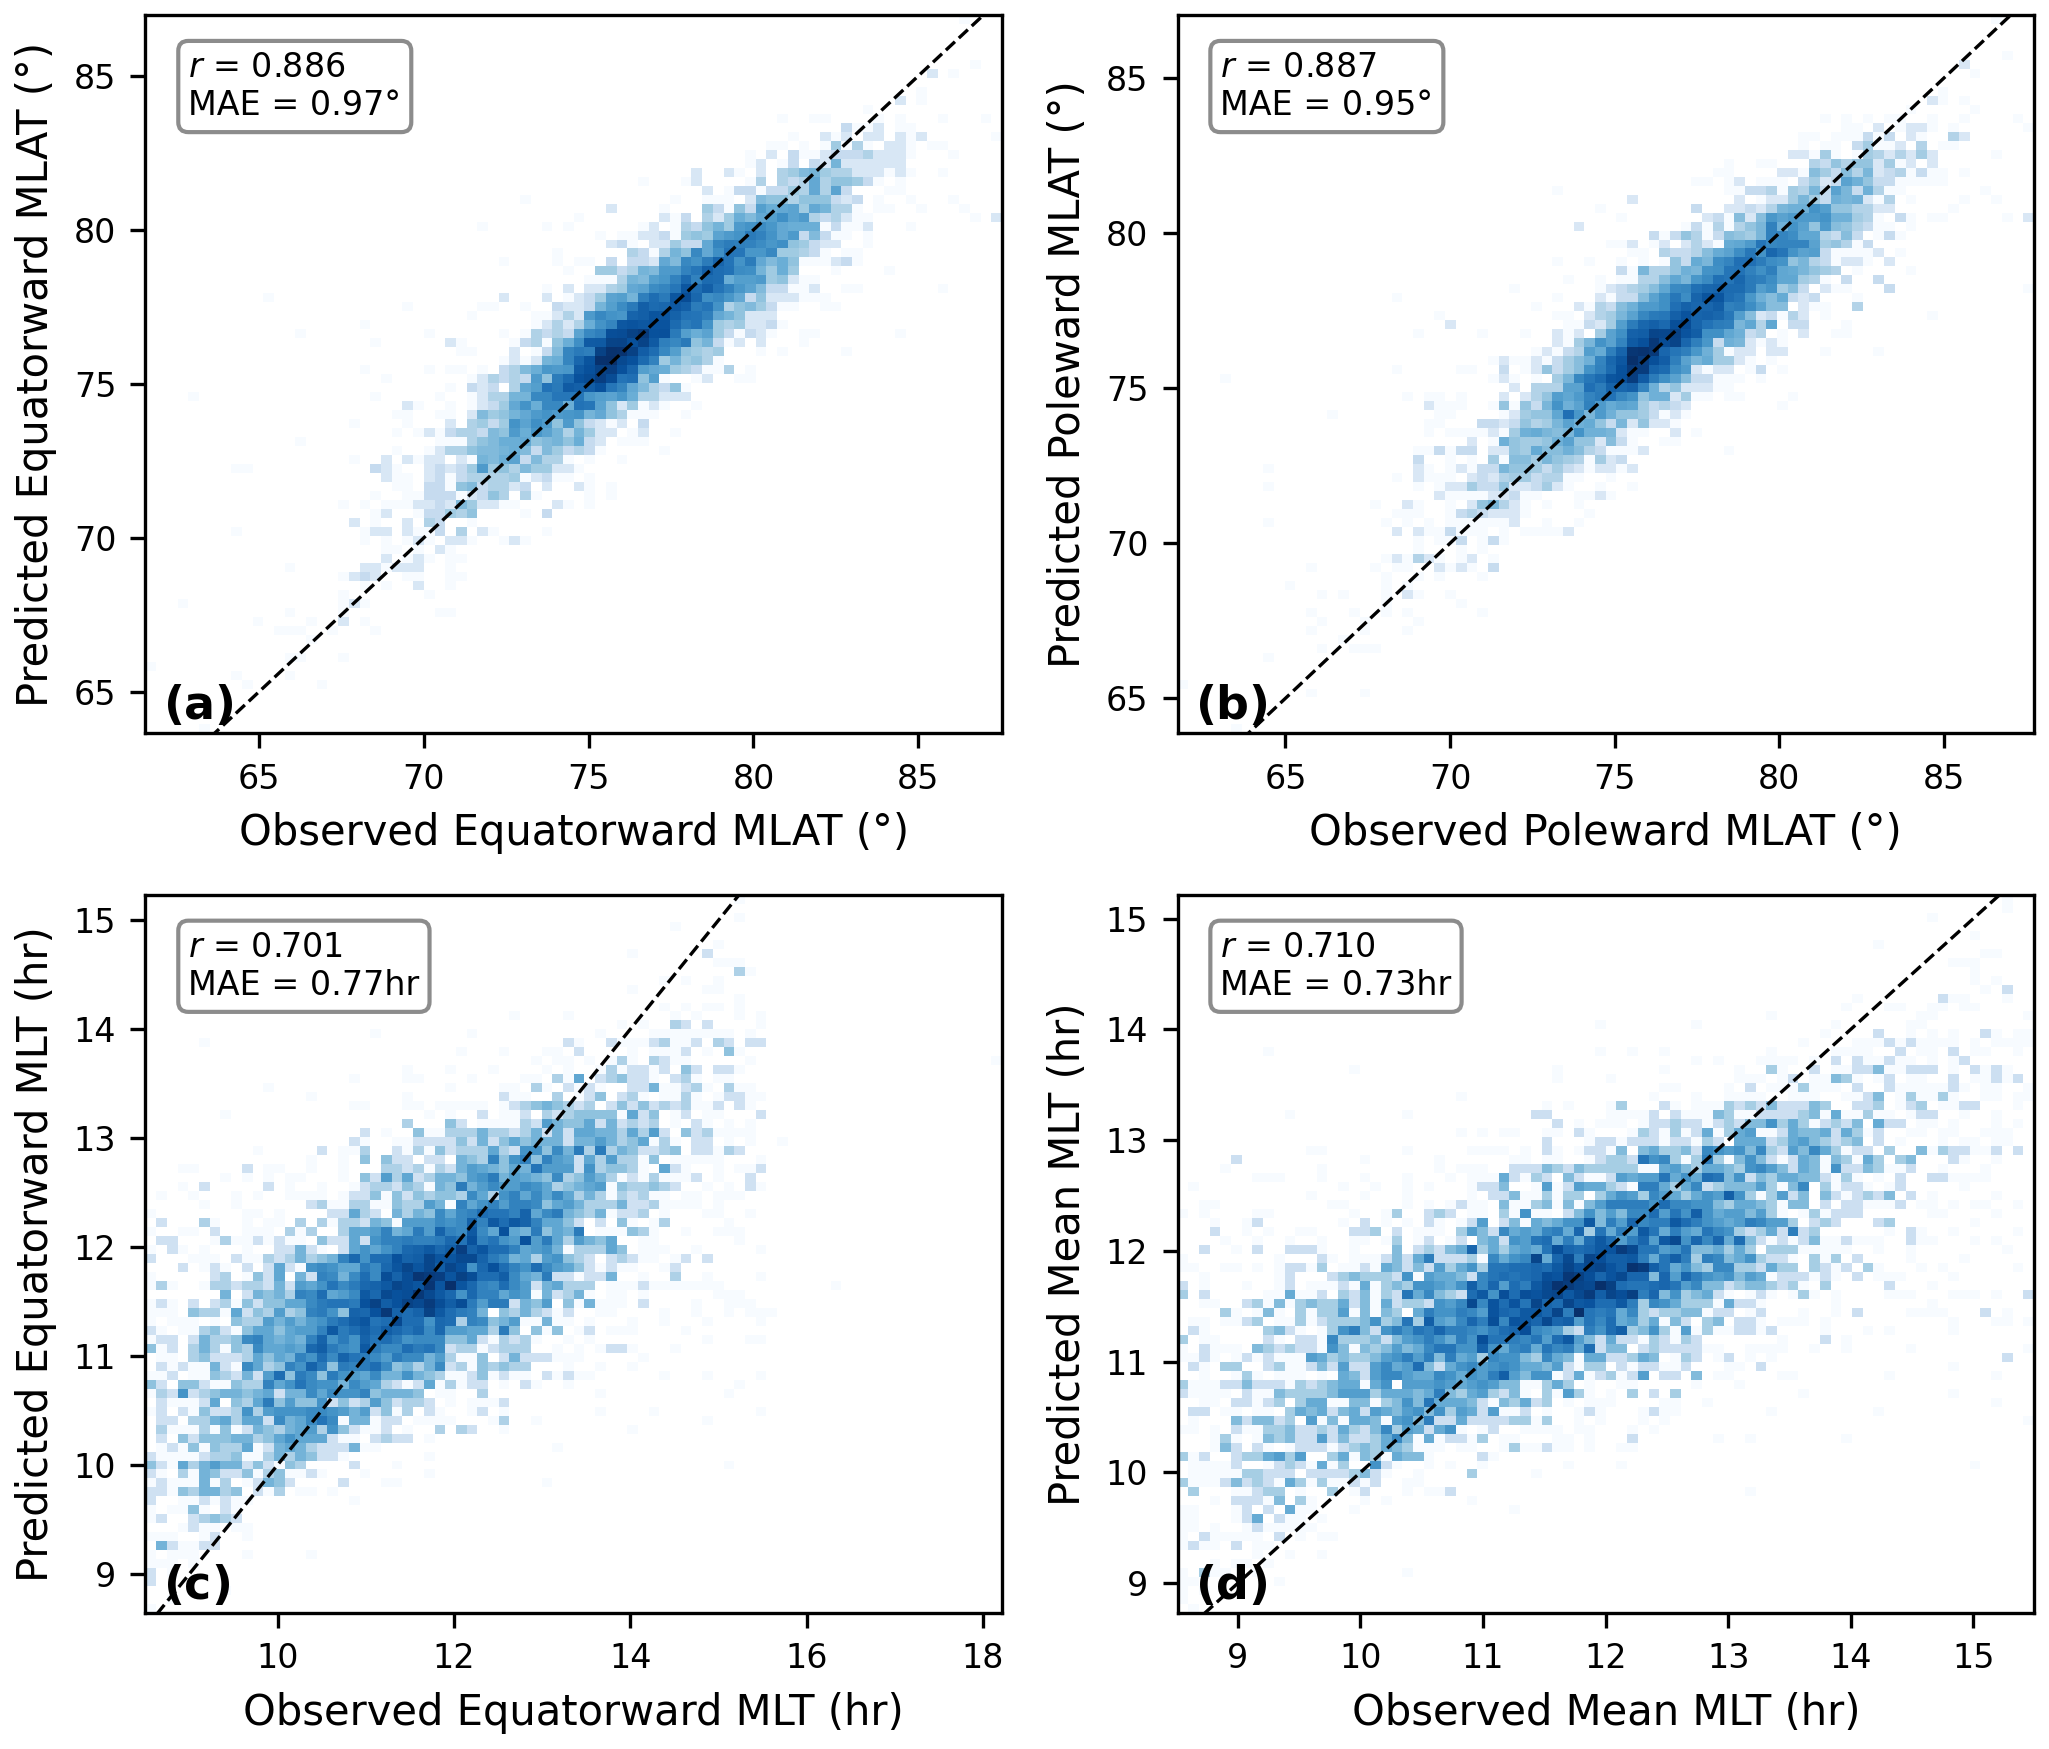
\includegraphics[width=\textwidth]{figures/fig02_scatter_4panel.png}
\caption{Predicted versus observed values for all four cusp boundary parameters: (a) equatorward MLAT, (b) poleward MLAT, (c) equatorward MLT, and (d) mean MLT. Color indicates point density. The dashed line is the 1:1 line. Pearson $r$ and MAE are annotated in each panel.}
\label{fig:scatter}
\end{figure}

Figure~\ref{fig:baseline} lines up the equatorward MLAT MAE across models of increasing complexity. Starting from a single-variable linear fit on $B_z$ (MAE = 2.04\textdegree), switching to the Newell coupling function brings the MAE down to 1.80\textdegree. Fitting the same coupling function with Newell's nonlinear form ($\Lambda_c = a \, E_{WAV}^{2/3} + b$) offers almost no further gain: 1.80\textdegree, $r = 0.586$. XGBoost cuts the error nearly in half, to 0.97\textdegree{} on the test set---a 46\% drop. The 46\% MAE reduction under random splits persists as a 40\% reduction under temporal holdout (1.11\textdegree{} vs.\ 1.80\textdegree). Bootstrap resampling yields $[0.95, 0.99]$\textdegree{} CI for XGBoost ($p < 0.001$), though temporal autocorrelation among crossings means these CIs are likely too narrow. The widely cited $r = 0.78$--$0.83$ from \citet{newell2006cusp} were computed on \textit{binned} data; on individual crossings the Newell coupling function reaches only $r \approx 0.58$. Our $r = 0.887$ on individual crossings is considerably higher.

\begin{figure}[htbp]
\centering
\noindent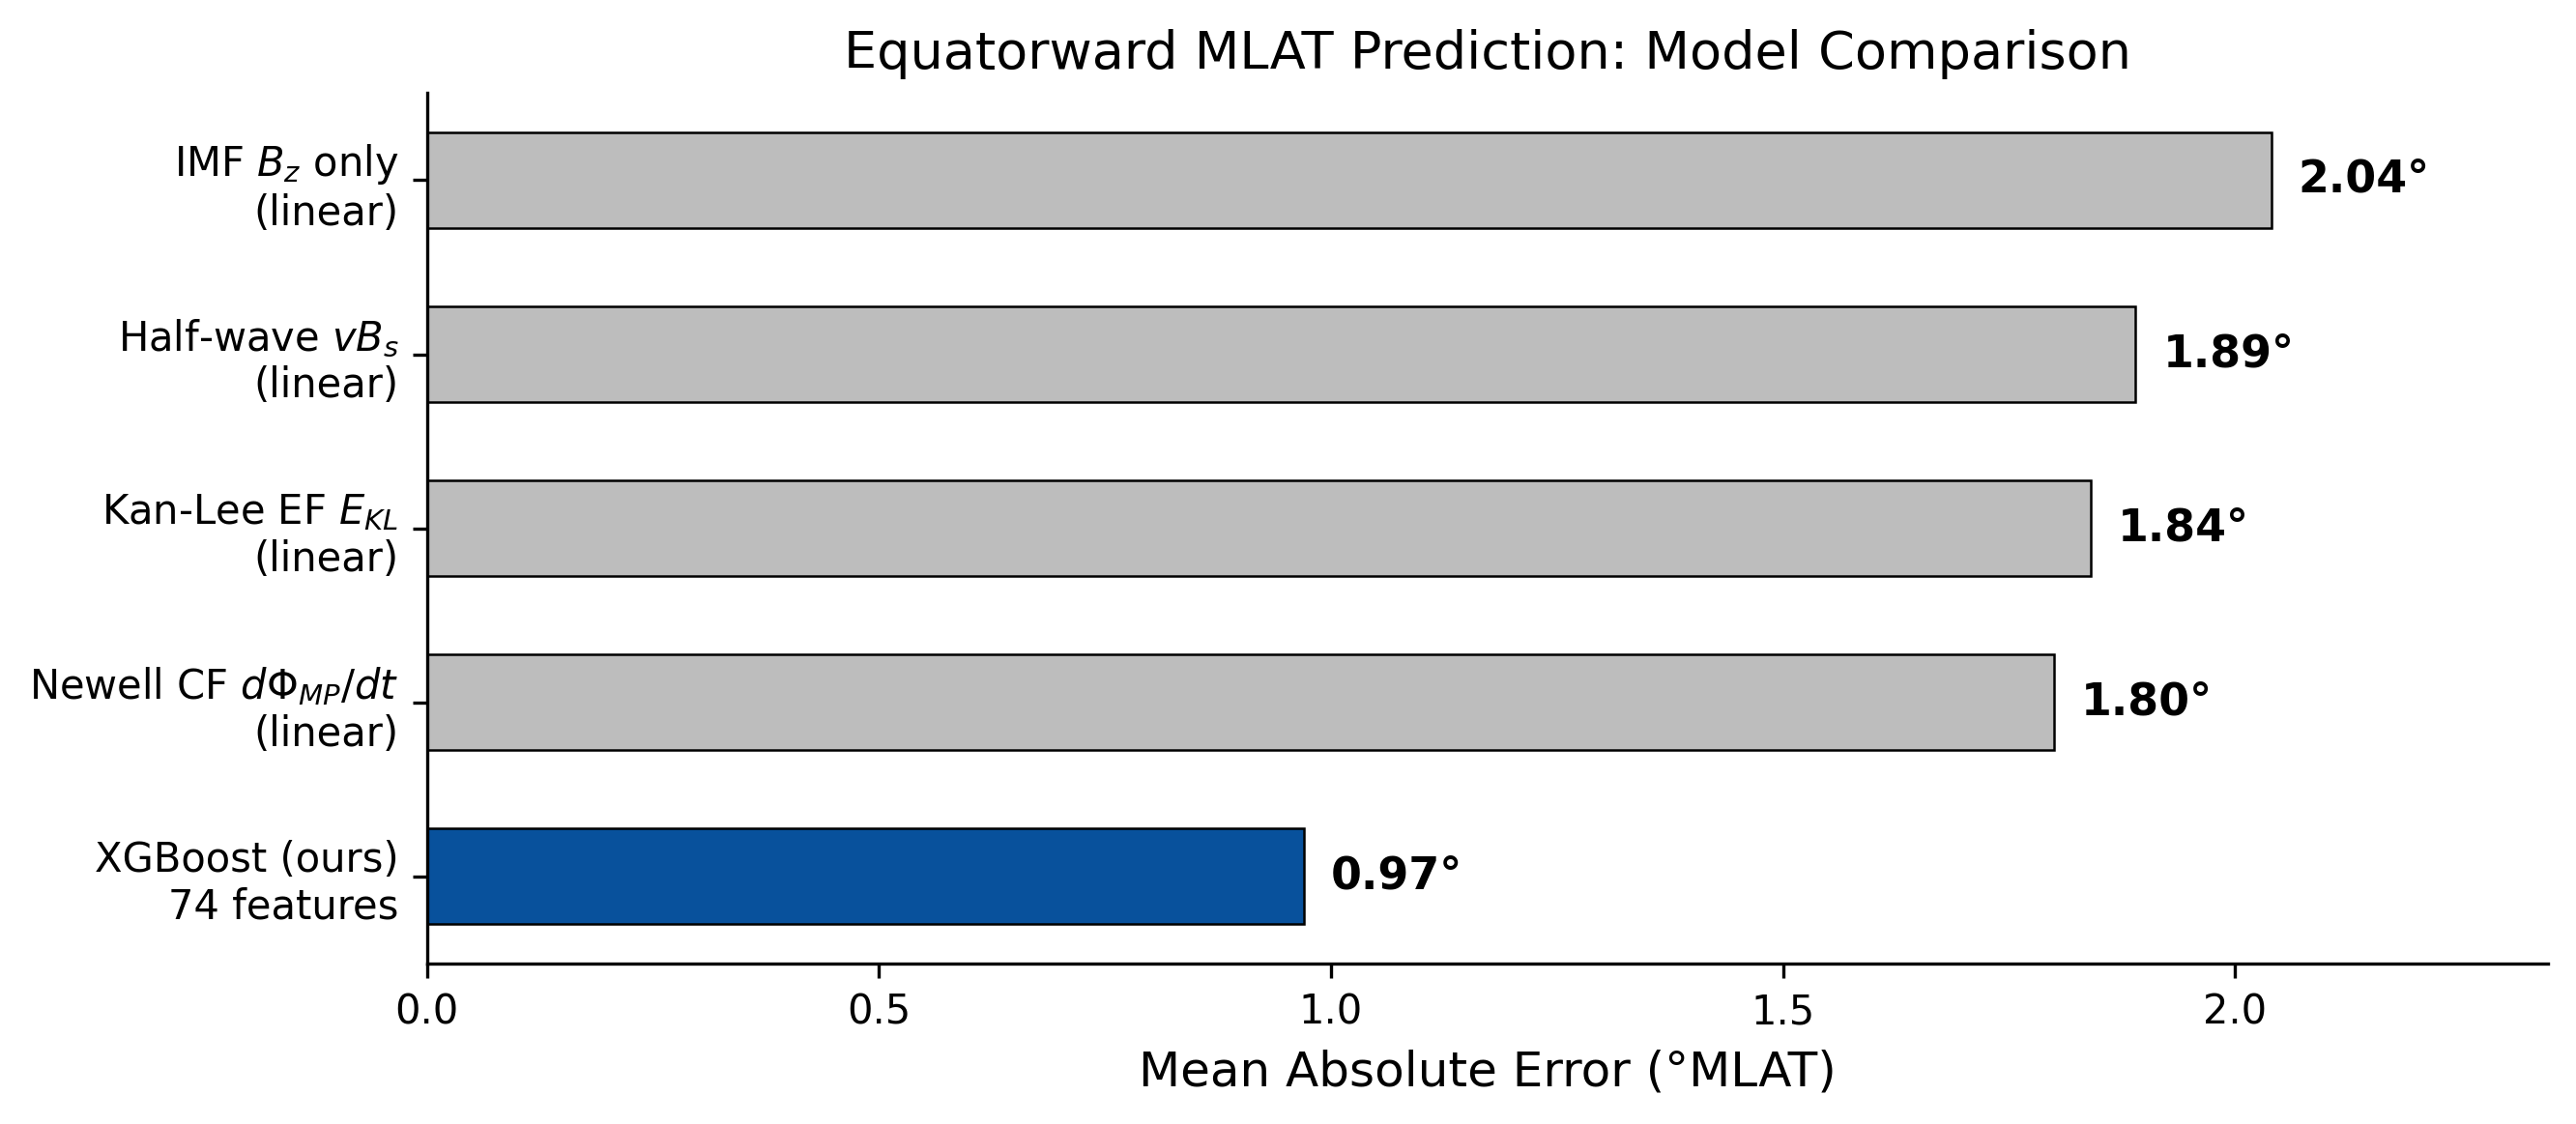
\includegraphics[width=0.6\textwidth]{figures/fig03_baseline_comparison.png}
\caption{Comparison of equatorward MLAT prediction accuracy (MAE in degrees) across baseline models and XGBoost. $B_z$ = IMF north-south component; $vB_s$ = half-wave rectified southward electric field ($v \cdot \max(-B_z, 0)$); Kan-Lee EF = Kan-Lee merging electric field ($E_{KL} = v B_T \sin^2(\theta_c/2)$; \citealt{kan1979reconnection}); Newell CF = Newell coupling function ($d\Phi_{MP}/dt$; \citealt{newell2007coupling}). All baselines use linear regression on a single predictor; XGBoost uses all 74 features.}
\label{fig:baseline}
\end{figure}

The residuals (Figure~\ref{fig:error_dist}) are roughly Gaussian, centered near zero (mean bias $< 0.03$\textdegree{} in magnitude, standard deviation 1.34\textdegree). Most predictions land close to the observations: 63\% within 1\textdegree, 89\% within 2\textdegree, and only 3\% exceed 3\textdegree. These errors should be interpreted in the context of the cusp's spatial scale: the full cusp region extends over $\sim$3--4\textdegree{} MLAT \cite{zhang2013lfm}, while the equatorward boundary itself varies over a $\sim$14\textdegree{} range (65--80\textdegree{}) depending on solar wind conditions.

\begin{figure}[htbp]
\centering
\noindent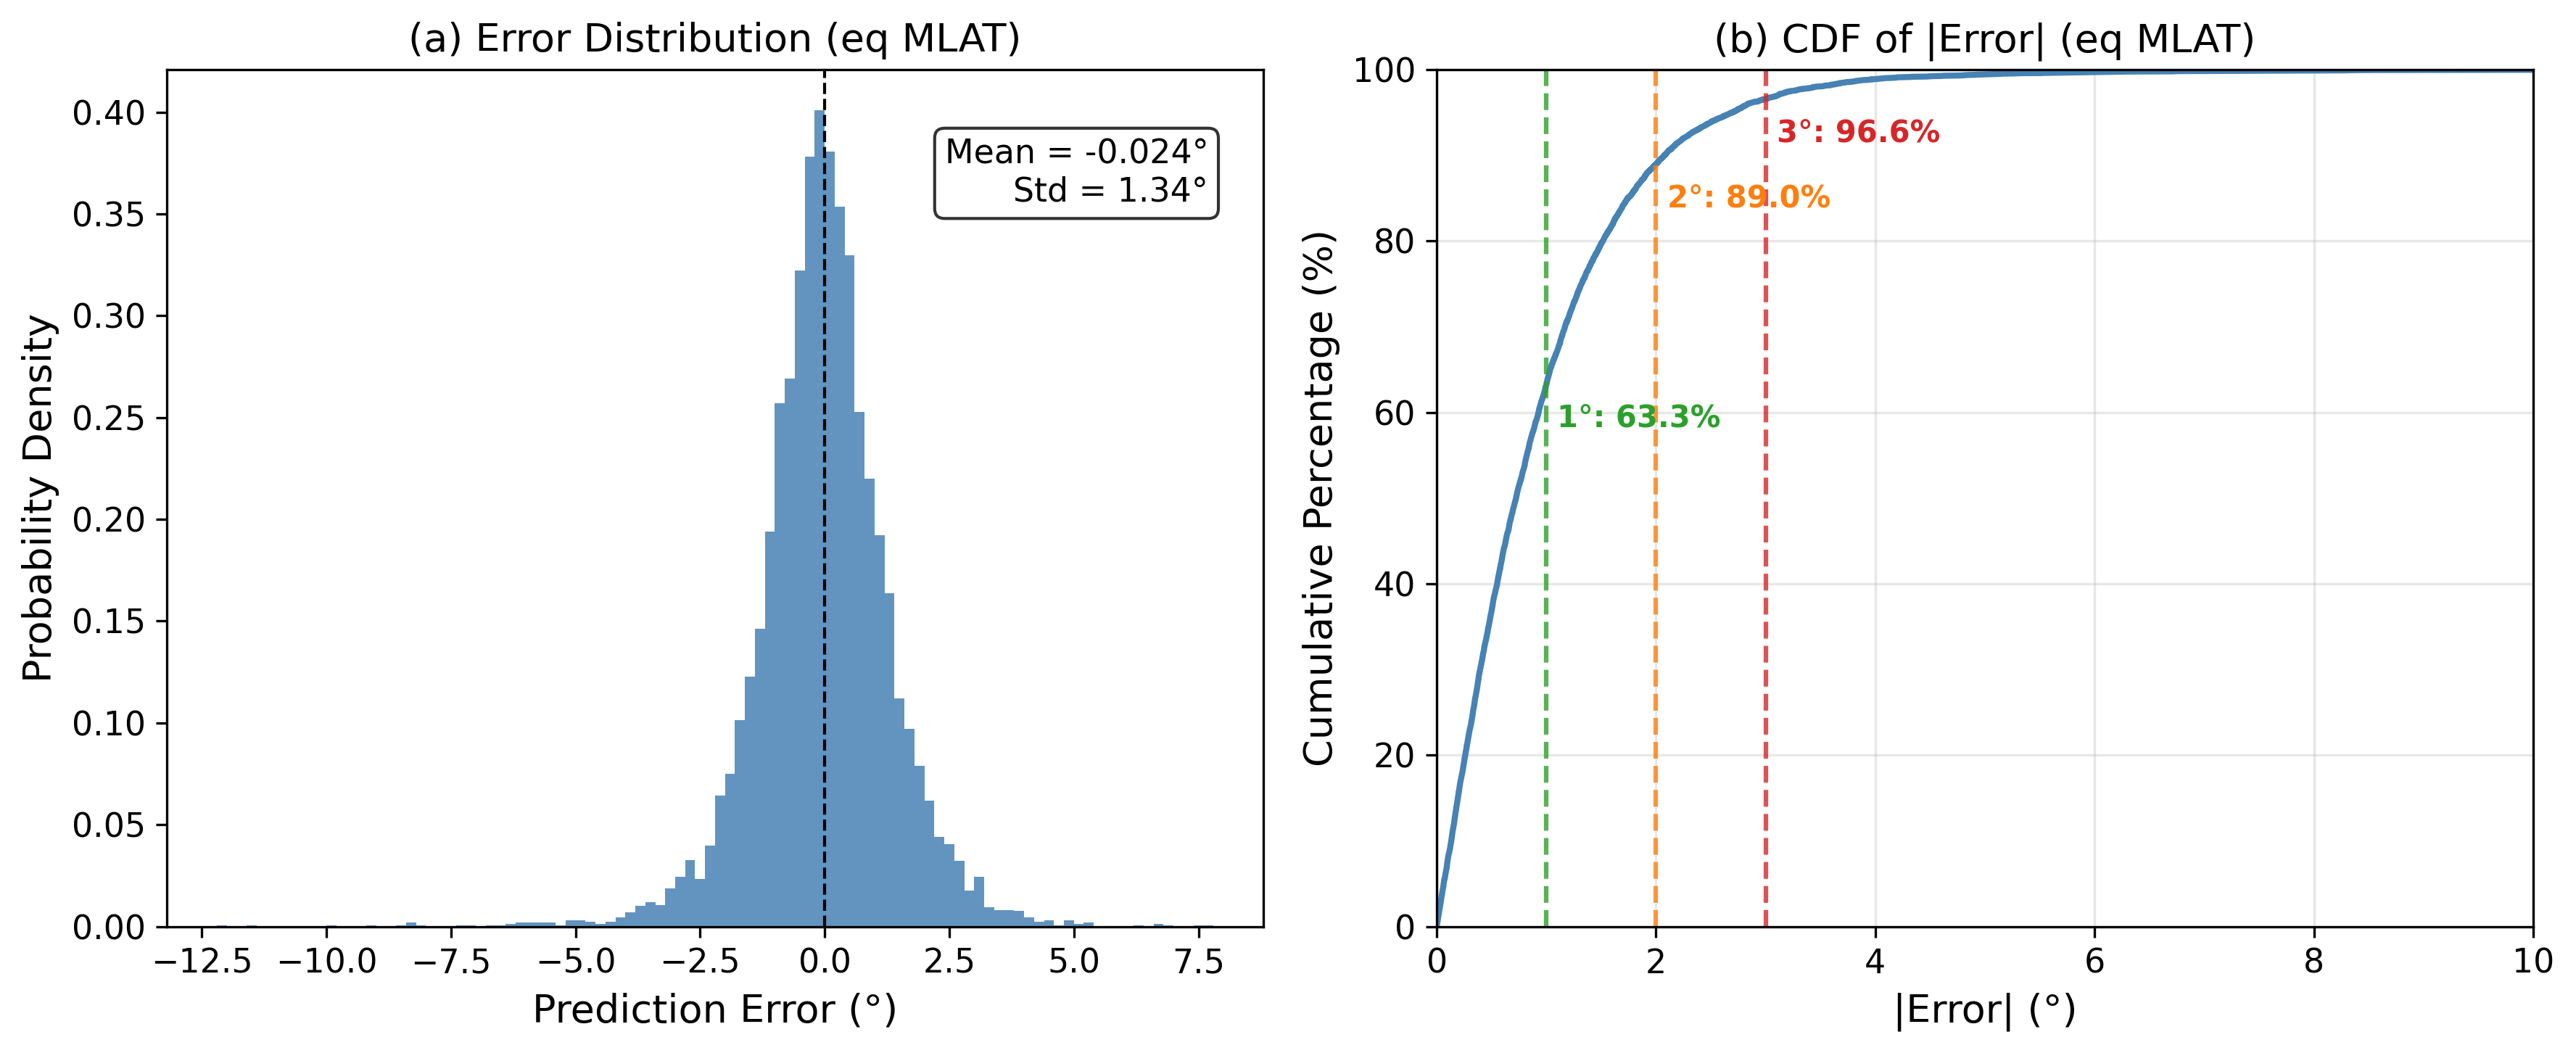
\includegraphics[width=0.75\textwidth]{figures/fig04_error_distribution.png}
\caption{Error analysis for equatorward MLAT prediction. (a) Distribution of prediction residuals (predicted $-$ observed). (b) Cumulative distribution of absolute errors, with vertical lines marking the 1\textdegree, 2\textdegree, and 3\textdegree{} thresholds and corresponding percentages.}
\label{fig:error_dist}
\end{figure}

\subsection{Feature Importance, Timescale Dependence, and Partial Dependence}

Figure~\ref{fig:importance} displays the gain-based feature importance for the top 20 features in the equatorward MLAT model. The 60-minute mean Newell coupling function (\texttt{newell\_cf\_mean60}) is the most important feature by gain, followed by $vB_s$ mean over 60 minutes, the 60-minute integral of $vB_s$, and the 60-minute integral of the Newell coupling function. Together, the four 60-minute coupling function features account for over 55\% of total gain-based importance. As a cross-check, we computed SHAP \citep{lundberg2017shap} values on 2{,}000 test-set samples. The SHAP ranking agrees with gain: the 60-minute mean coupling function has the largest mean absolute SHAP value (1.07\textdegree), followed by dipole tilt (0.32\textdegree) and 15-minute mean $B_z$ (0.23\textdegree). Gain-based importance can overweight features with high cardinality, so this agreement lends confidence to the ranking.

\begin{figure}[htbp]
\centering
\noindent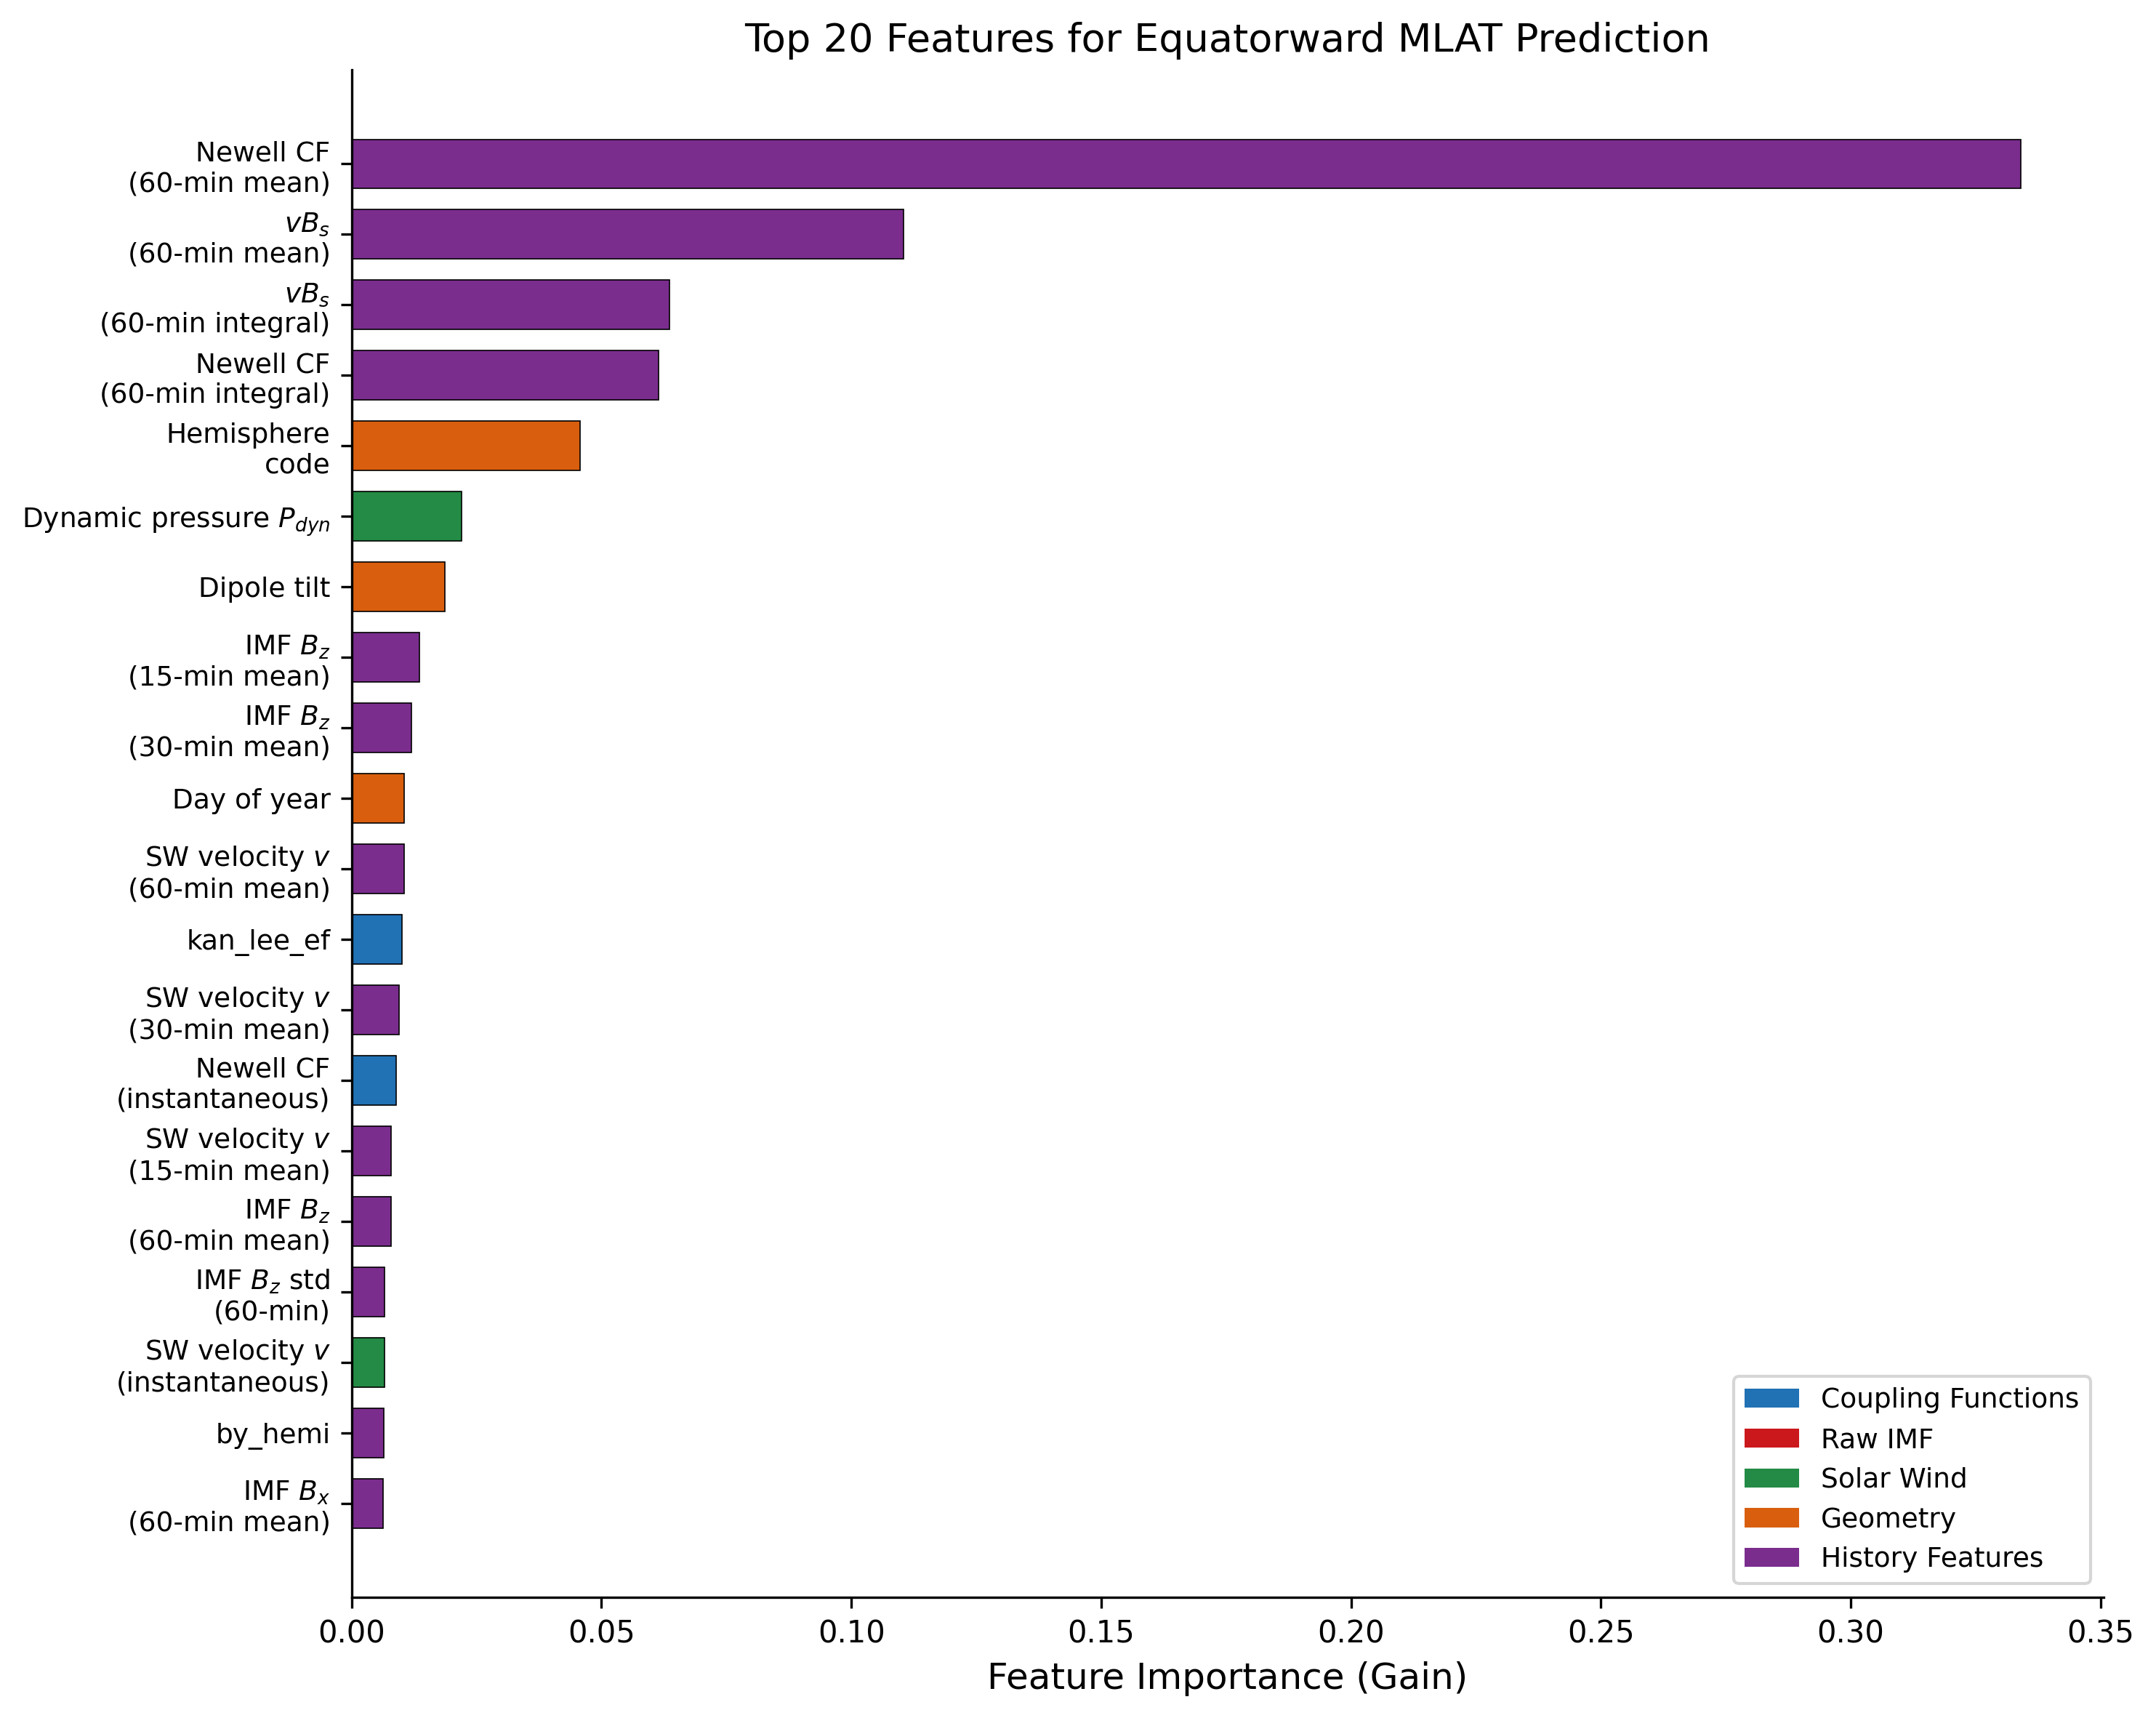
\includegraphics[width=0.65\textwidth]{figures/fig05_feature_importance.png}
\caption{Top 20 features for equatorward MLAT prediction, ranked by gain-based importance. Feature names indicate the physical quantity and averaging window (e.g., ``Newell CF (60-min mean)'' = 60-minute mean of the Newell coupling function $d\Phi_{MP}/dt$; ``$vB_s$ (60-min integral)'' = time-integrated half-wave rectified southward electric field). Colors indicate category: coupling functions (blue), raw IMF (red), solar wind (green), geometry (orange), and history features (purple).}
\label{fig:importance}
\end{figure}

The dominance of 60-minute features is confirmed by an ablation experiment (Figure~\ref{fig:timescale}). With instantaneous features alone the MAE is 1.27\textdegree. Adding 15 minutes of history drops it to 1.08\textdegree; 30 minutes reaches 1.02\textdegree; and 60 minutes gets to 0.99\textdegree. Combining all three windows (the full 74-feature model) adds little over the 60-minute-only result: 0.97\textdegree{} versus 0.99\textdegree. The 60-minute window clearly dominates, in line with the $\sim$1-hour magnetospheric reconfiguration timescale \cite{burton1975dst, newell2006cusp}.

\begin{figure}[htbp]
\centering
\noindent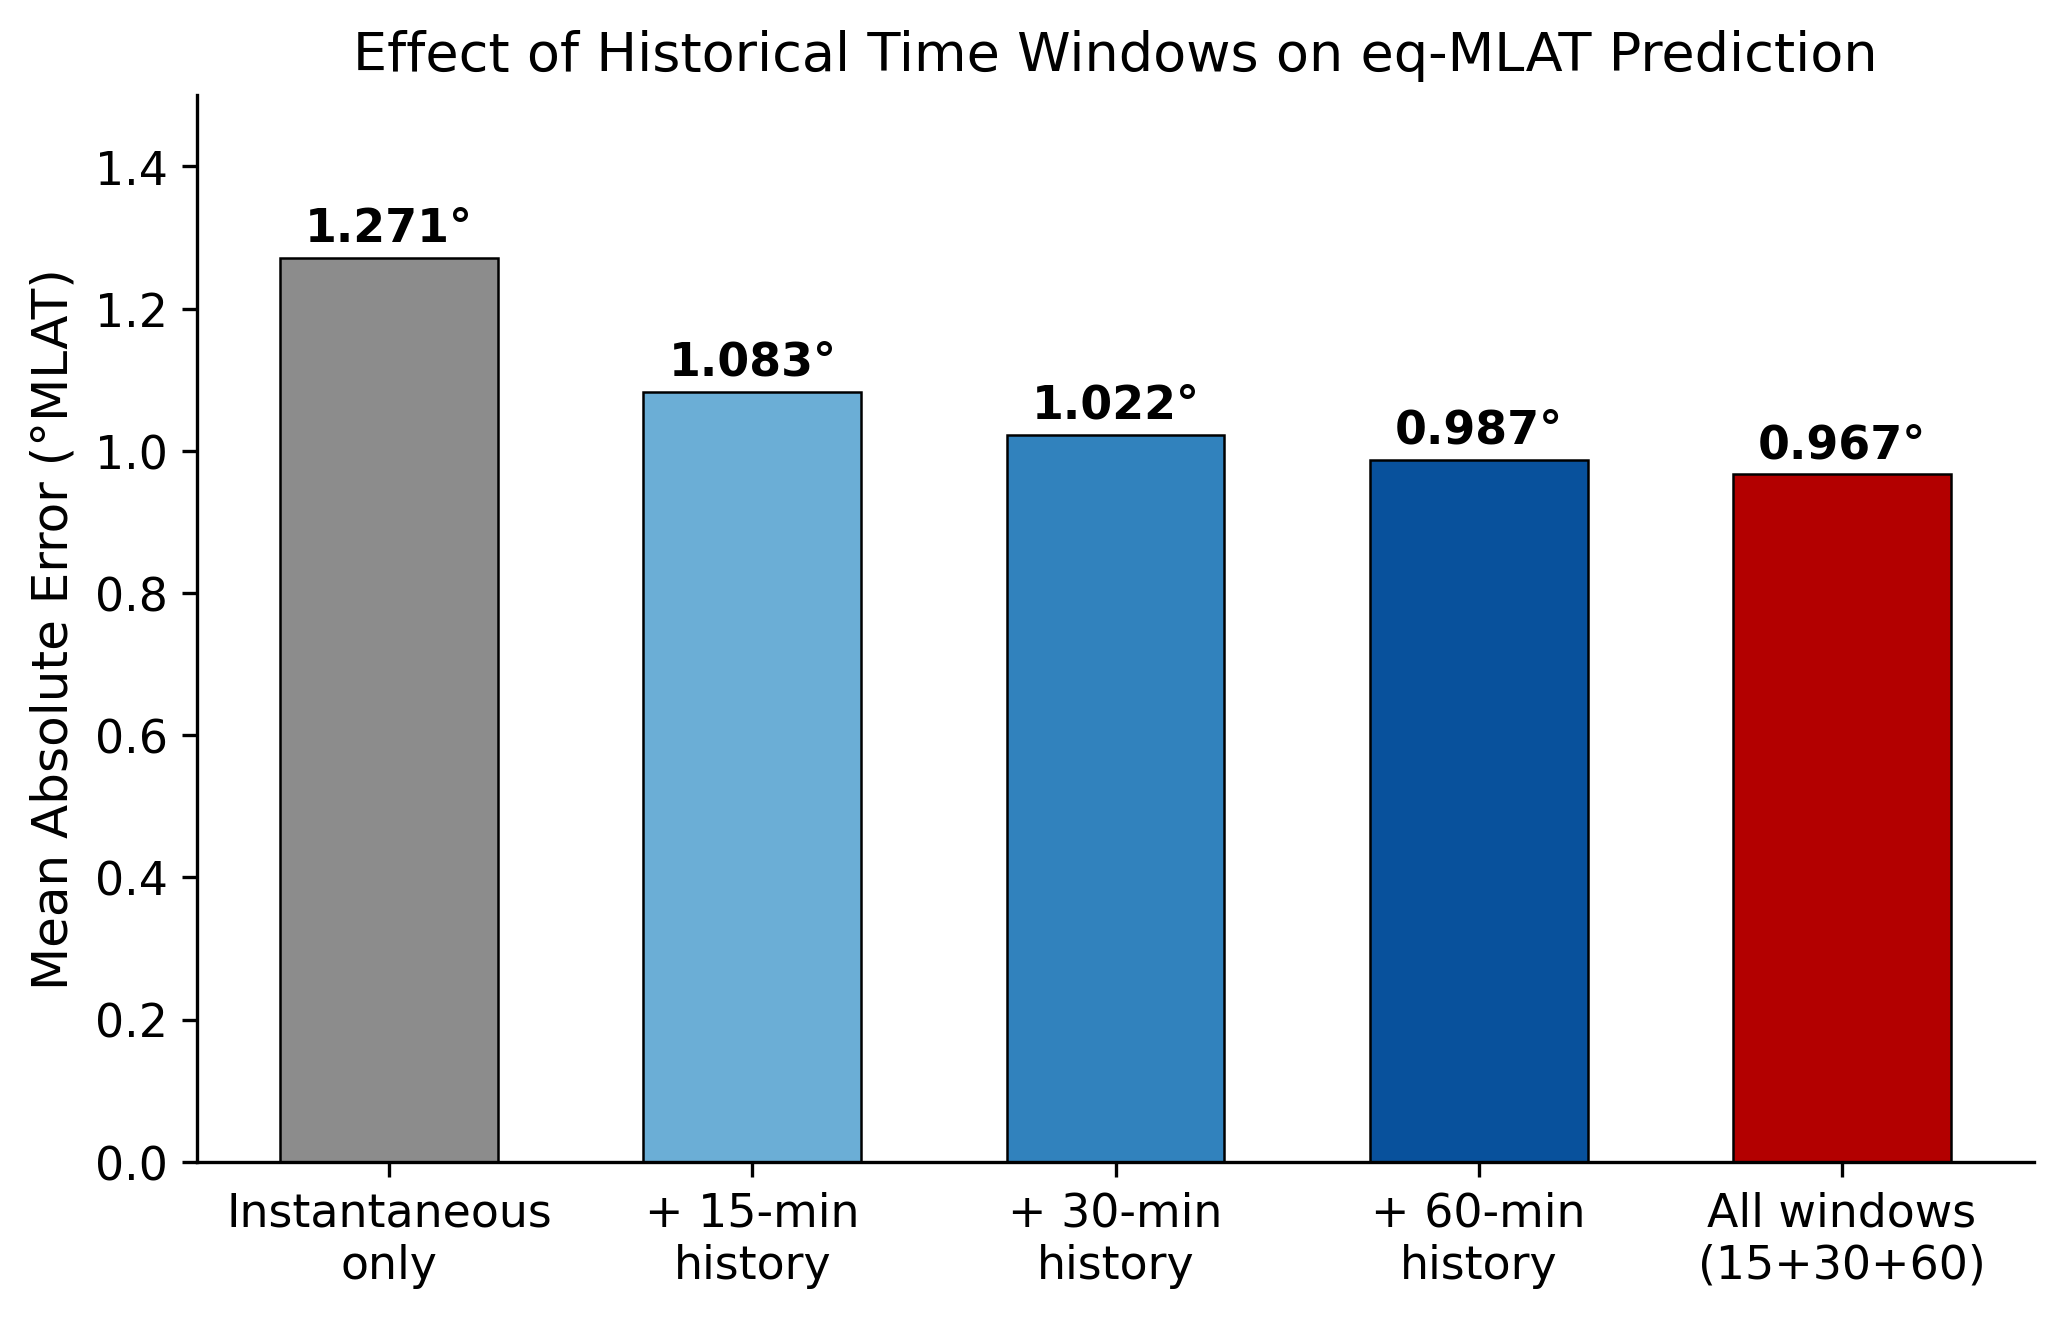
\includegraphics[width=0.6\textwidth]{figures/fig06_time_window_comparison.png}
\caption{Effect of historical time windows on equatorward MLAT prediction MAE. Each bar represents a model trained with the indicated feature set. The 60-minute history provides the largest improvement over instantaneous-only features.}
\label{fig:timescale}
\end{figure}

Figure~\ref{fig:partial_dep} shows partial dependence plots for six key features, revealing the marginal effect of each variable on the predicted equatorward MLAT (after averaging over all other features). The partial dependence on dipole tilt (panel a) shows a negative slope of approximately $-0.05$\textdegree/\textdegree, in excellent agreement with the $-0.06$\textdegree/\textdegree{} reported by \citet{newell1989tilt} and the $-0.046$\textdegree/\textdegree{} found by \citet{anderson2024cusp} for the Northern Hemisphere. The dependence on the 60-minute Newell coupling function (panel b) is strongly nonlinear, consistent with the $E_{WAV}^{2/3}$ dependence found by \citet{newell2006cusp}: the cusp moves equatorward rapidly at low coupling function values and saturates at high values. The IMF $B_z$ dependence (panel c) shows the expected asymmetry, with strong equatorward displacement for southward IMF ($B_z < 0$) and weak poleward return for northward IMF. Dynamic pressure (panel d) produces a weak equatorward shift at high values, consistent with magnetopause compression \cite{shue1997magnetopause}. The IMF $B_y$ dependence (panel e) is approximately symmetric around zero, as expected since $B_y$ primarily affects MLT rather than MLAT. The $vB_s$ dependence (panel f) shows a monotonically increasing equatorward displacement with increasing half-wave-rectified southward IMF driving.

\begin{figure}[htbp]
\centering
\noindent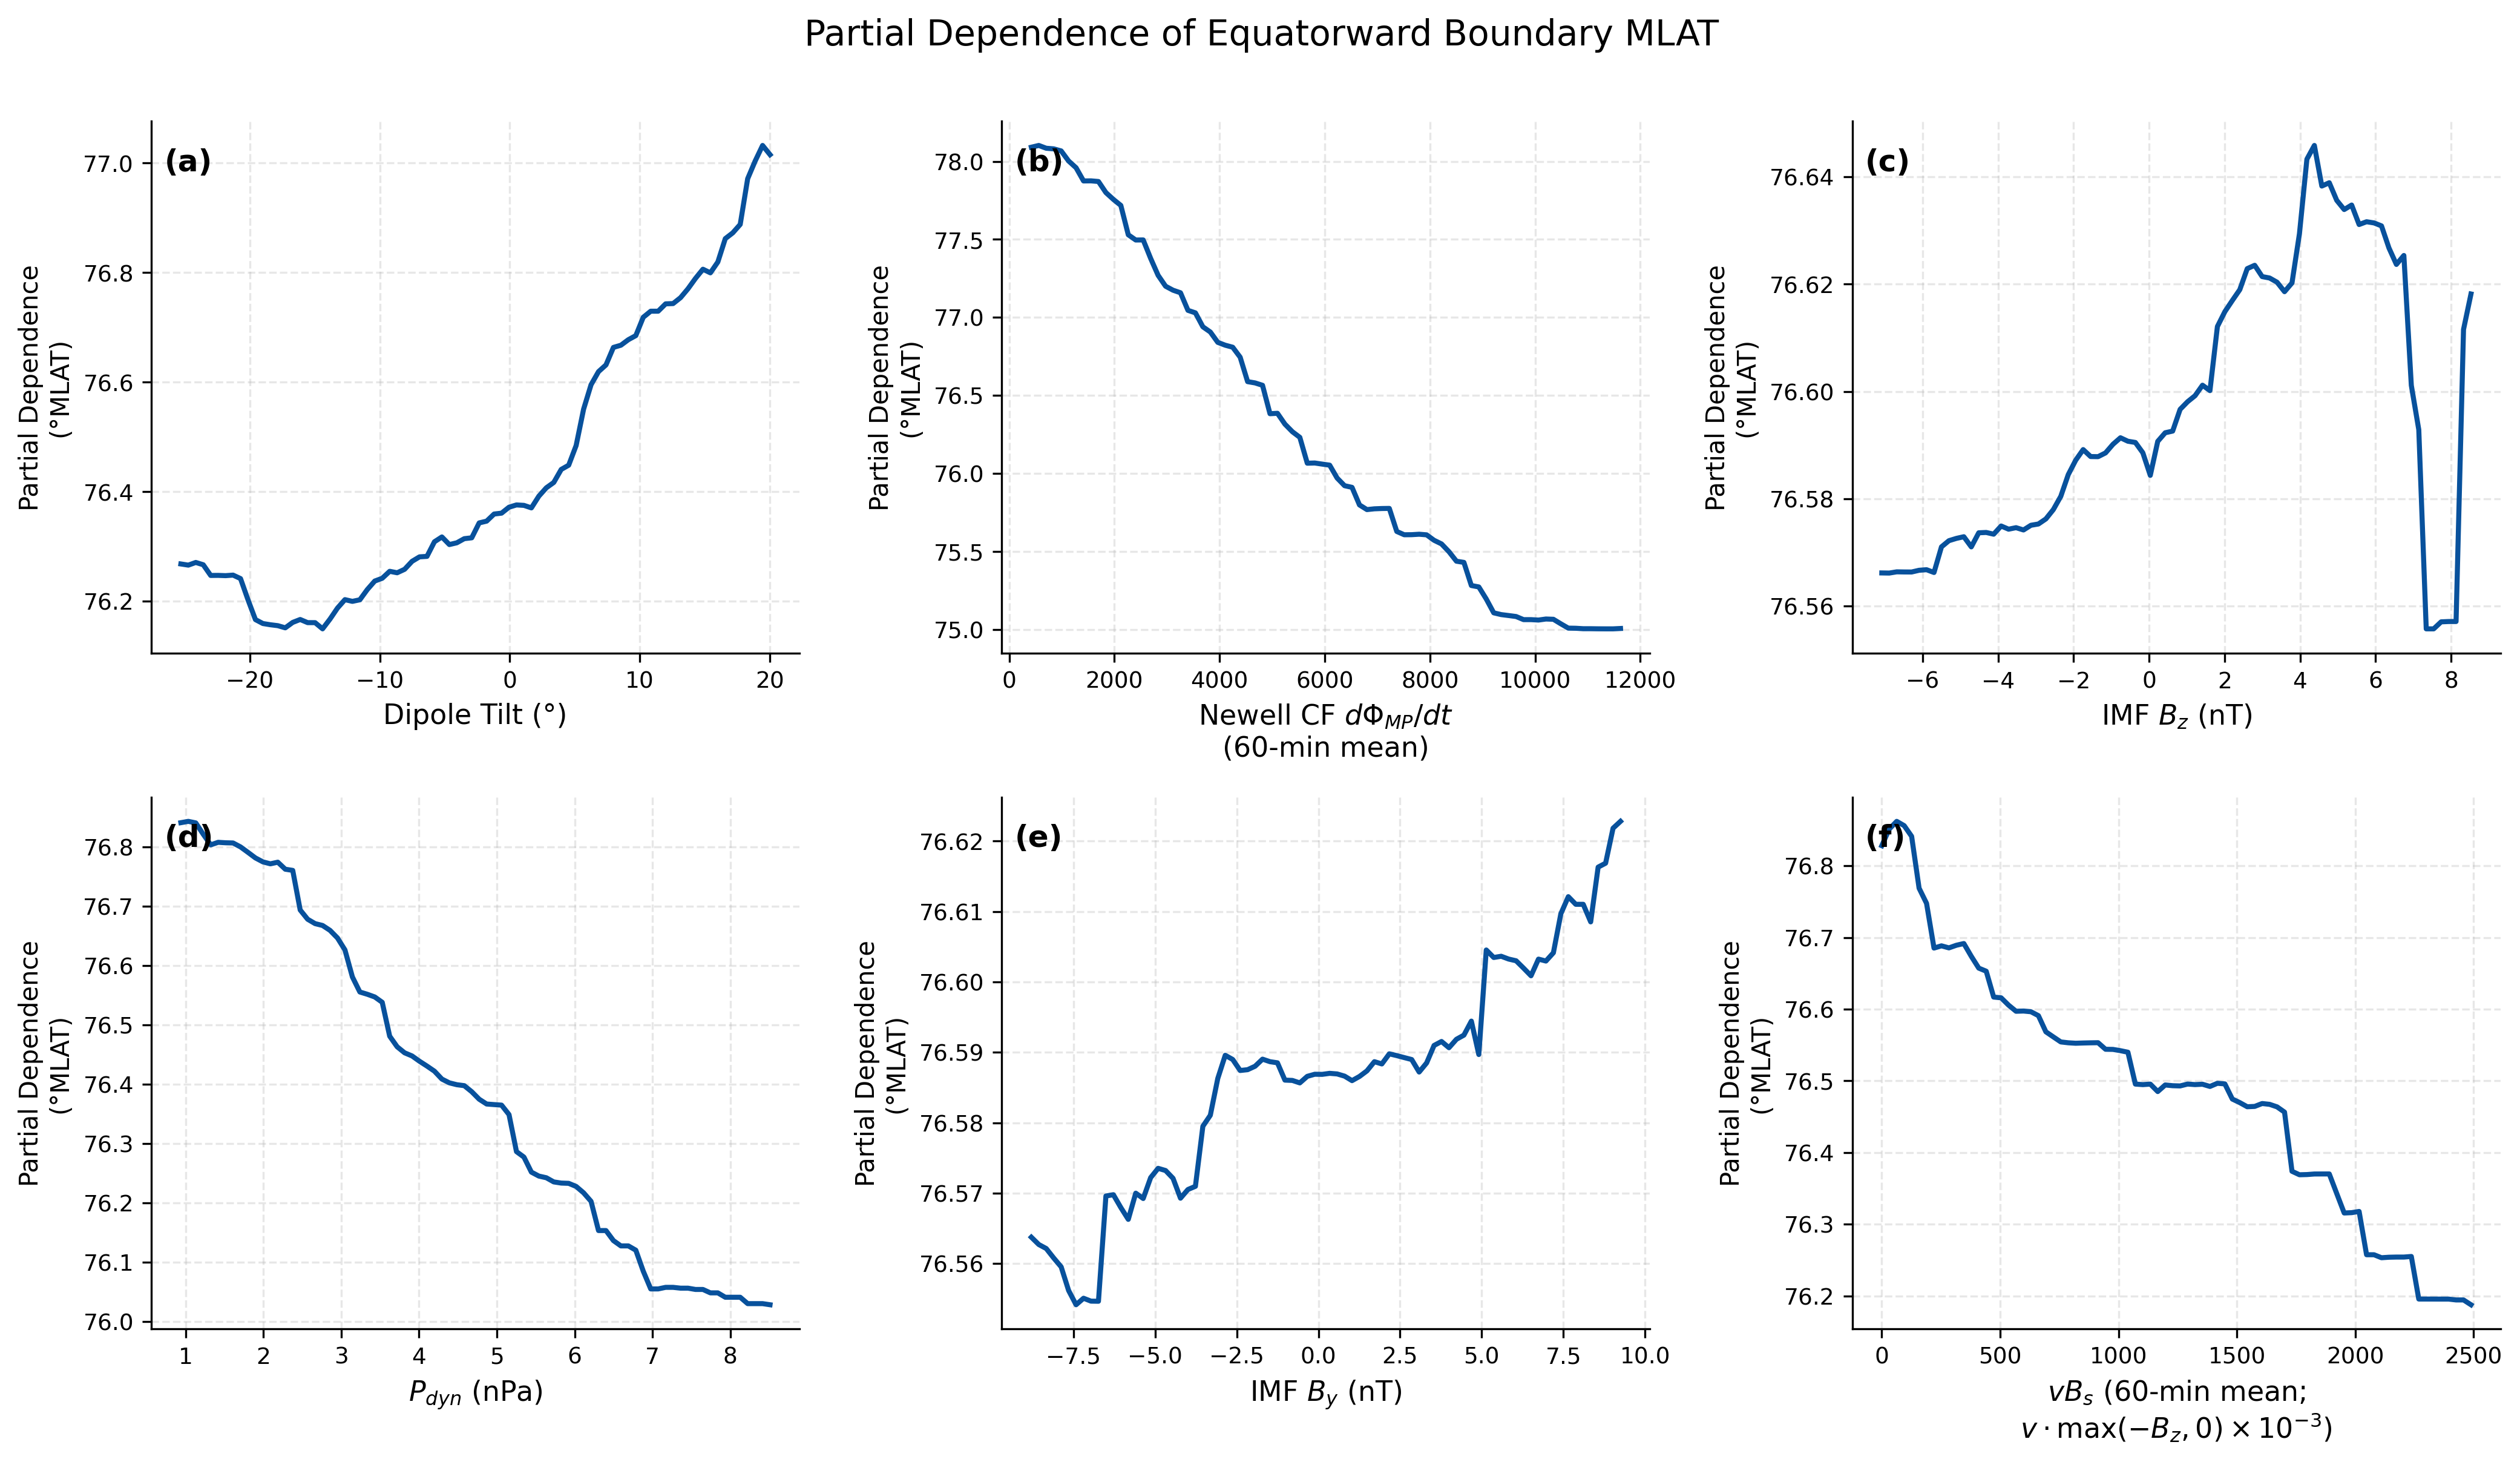
\includegraphics[width=0.9\textwidth]{figures/fig07_partial_dependence.png}
\caption{Partial dependence plots showing the marginal effect of six key features on predicted equatorward MLAT. (a) Dipole tilt, (b) 60-min mean Newell coupling function, (c) IMF $B_z$, (d) dynamic pressure, (e) IMF $B_y$, (f) 60-min mean $vB_s$.}
\label{fig:partial_dep}
\end{figure}

\subsection{Model Architecture Comparison}

Figure~\ref{fig:model_comp} compares the equatorward MLAT MAE across the structured baseline ladder, with all tree-based models evaluated on the same 39,668-sample dataset (80/20 random split, \texttt{random\_state=42}). The single-predictor Newell baseline achieves MAE = 1.80\textdegree. Ridge regression ($\ell_2$-regularized linear regression, $\alpha = 1.0$) on the same 74-feature input set achieves MAE = 1.41\textdegree{}---a 22\% improvement attributable to feature richness alone. The switch from Ridge to GBR-300 (300-tree gradient boosting, depth 5) further reduces MAE to 1.11\textdegree{} (21\% additional reduction), quantifying the contribution of nonlinear modeling. XGBoost-1000 achieves MAE = 0.97\textdegree{}, an additional 13\% improvement over GBR-300 attributable to deeper trees and extended boosting rounds. In total, XGBoost reduces MAE by 46\% relative to the Newell baseline.

Neural network architectures were evaluated on the \texttt{omni\_hist} subset ($\sim$11,700 samples) during architecture search. The TabTransformer (d128, 2 layers) achieved MAE = 1.11\textdegree{}, the ResMLP (4 blocks, 128 hidden units) achieved MAE = 1.02\textdegree{}, and the standard MLP with GeLU activation achieved MAE = 1.53\textdegree{}. These results are not directly comparable to the tree-based models due to the smaller evaluation dataset; nonetheless, even the best neural architecture (ResMLP, 1.02\textdegree{}) does not reach XGBoost-1000 (0.97\textdegree{}) performance, consistent with the established advantage of gradient-boosted trees for tabular data \citep{grinsztajn2022tree}.

\begin{figure}[htbp]
\centering
\noindent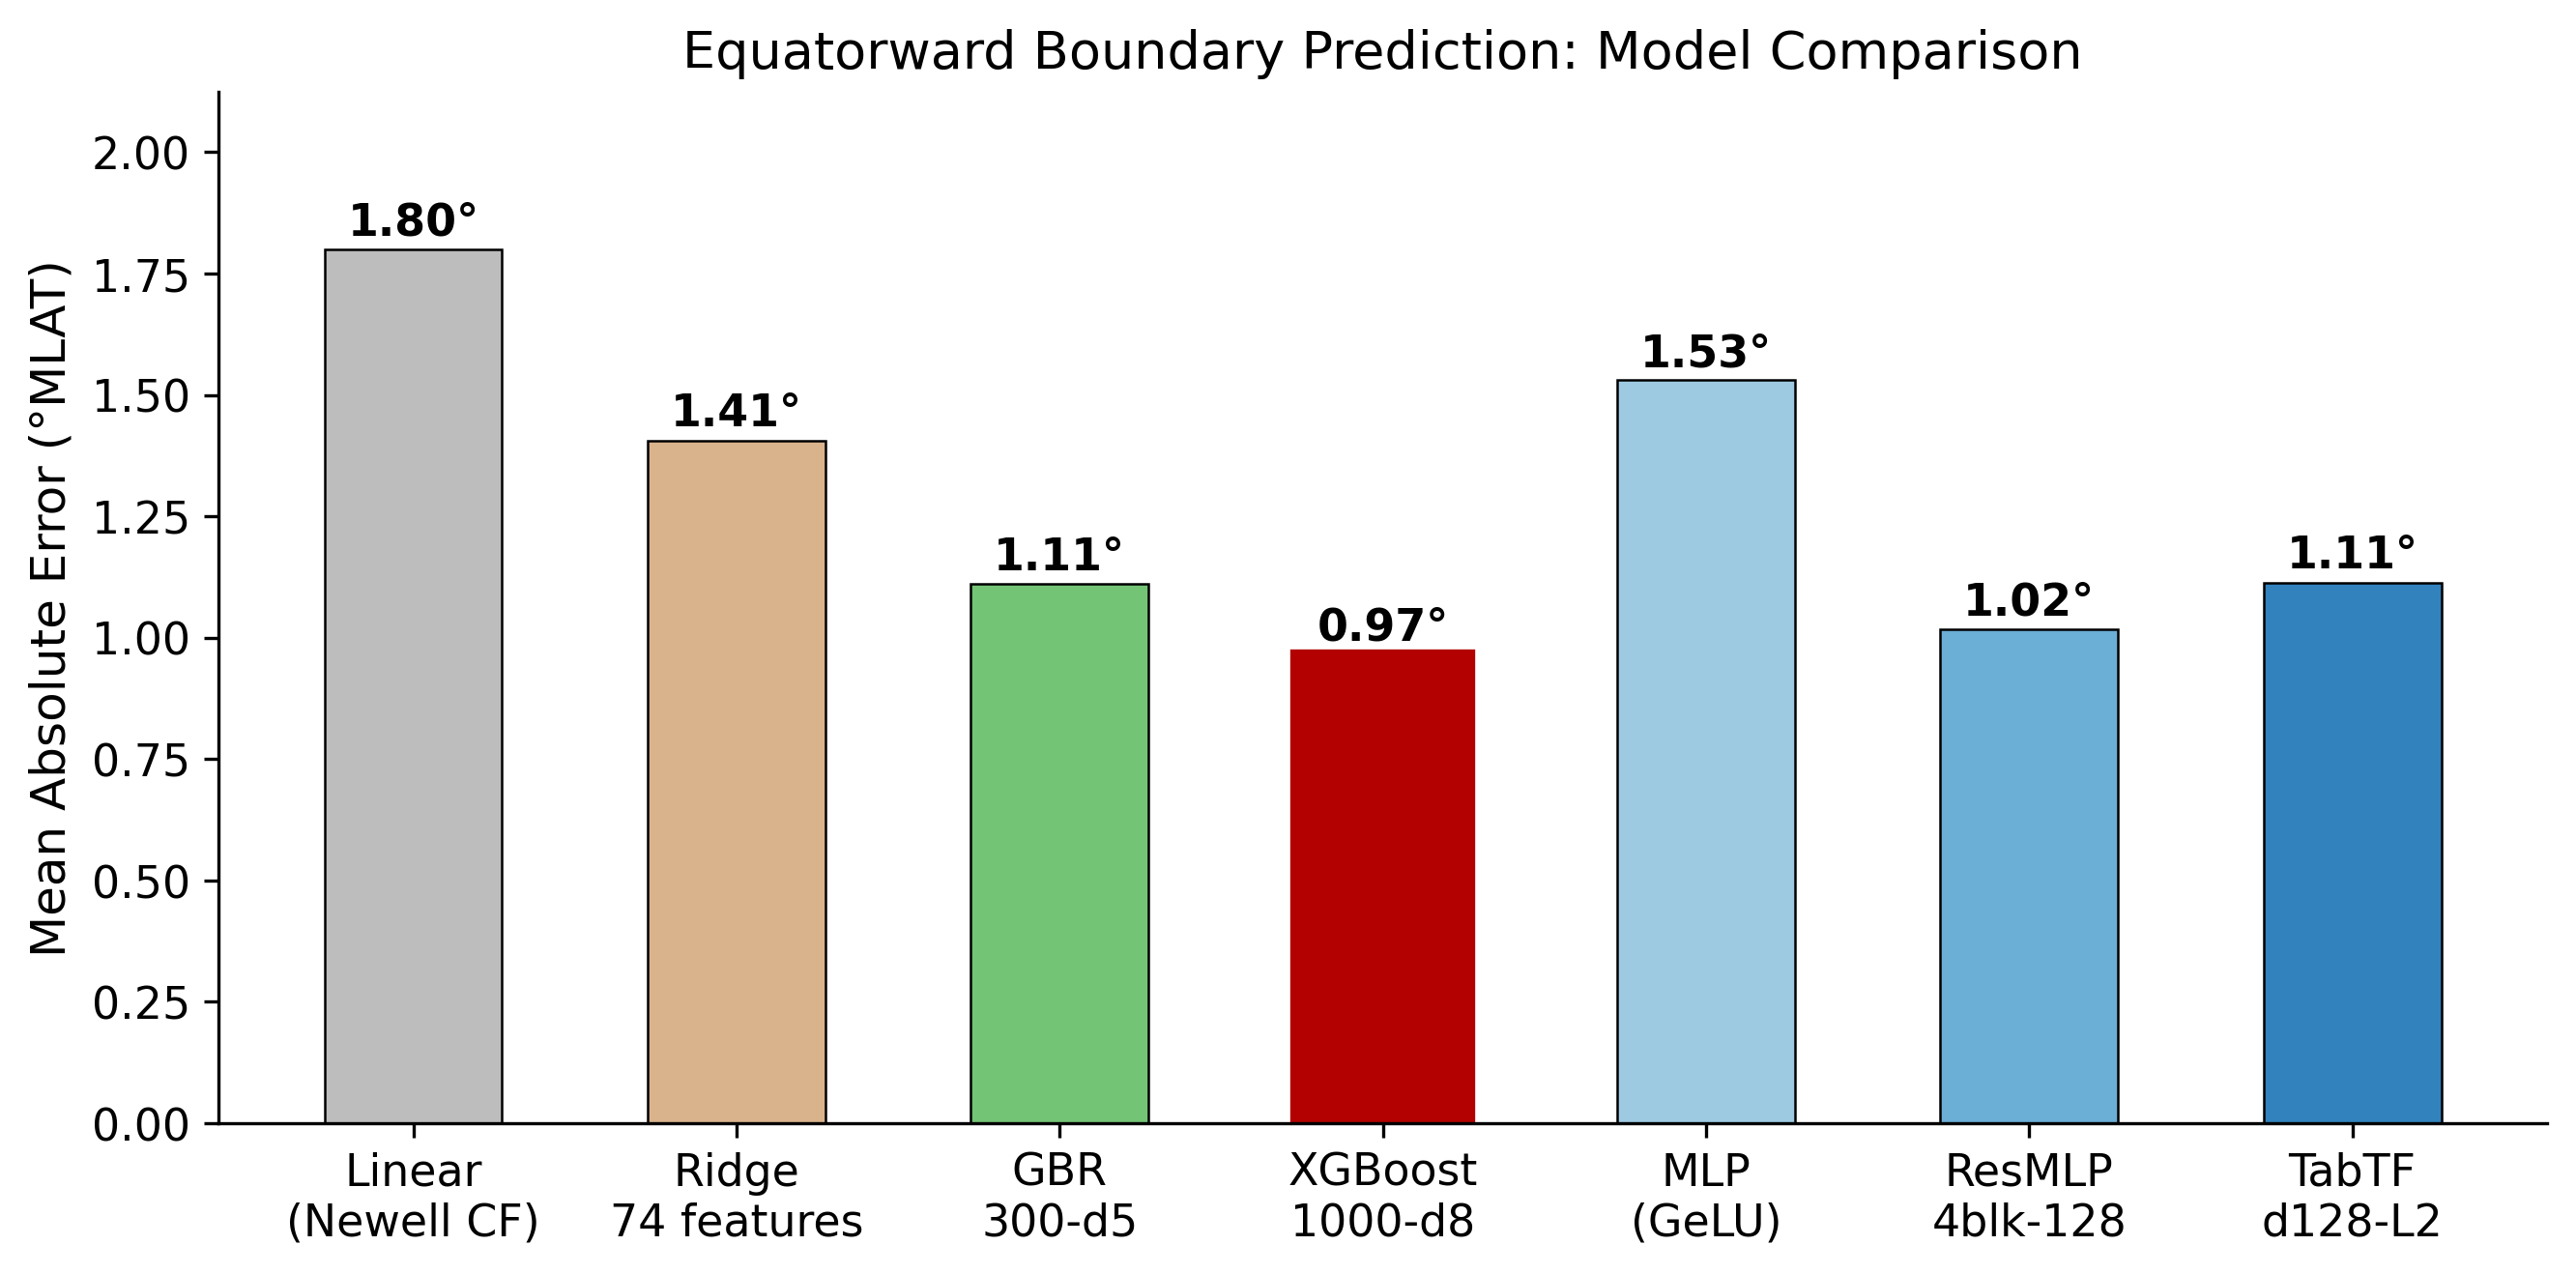
\includegraphics[width=0.6\textwidth]{figures/fig09_model_comparison.png}
\caption{Model architecture comparison for equatorward MLAT prediction. Bars show MAE (degrees). Tree-based models (Newell CF, Ridge, GBR-300, XGBoost-1000) are evaluated on the full 39,668-sample test set; neural network results are from an independent architecture search on a smaller subset ($\sim$11,700 samples). XGBoost-1000 achieves the lowest MAE overall.}
\label{fig:model_comp}
\end{figure}

\subsection{Robustness and Generalization}

\textbf{Hemispheric and geomagnetic activity dependence.} Figure~\ref{fig:hemi_ae} examines model performance across hemispheres and geomagnetic activity levels. The Northern Hemisphere ($n \approx 7{,}180$ test samples, 90\% of the test set) achieves MAE = 0.93\textdegree{} and $r = 0.889$, while the Southern Hemisphere ($n \approx 754$ test samples, 10\%) achieves MAE = 1.29\textdegree{} and $r = 0.865$ (panels a--b). The higher Southern Hemisphere MAE partly reflects the smaller training sample size in that hemisphere, which constitutes only $\sim$10\% of all DMSP cusp crossings in the dataset. Panel (c) shows that performance degrades during high auroral/substorm activity (AE $\geq 500$~nT), where MAE increases to 1.16\textdegree---a 25\% degradation relative to moderate activity (100--300~nT; MAE = 0.92\textdegree). The higher MAE during disturbed conditions has several likely sources: rapid magnetopause erosion \citep{pitout2021cluster}, flux transfer events that produce minute-scale boundary jumps, and amplified OMNI propagation uncertainty \citep{lockwood2022pitfalls}. Despite these challenges, the model still achieves MAE $\approx 1.16$\textdegree{} during high-activity intervals---well below the linear baseline MAE of 1.80\textdegree.

\begin{figure}[htbp]
\centering
\noindent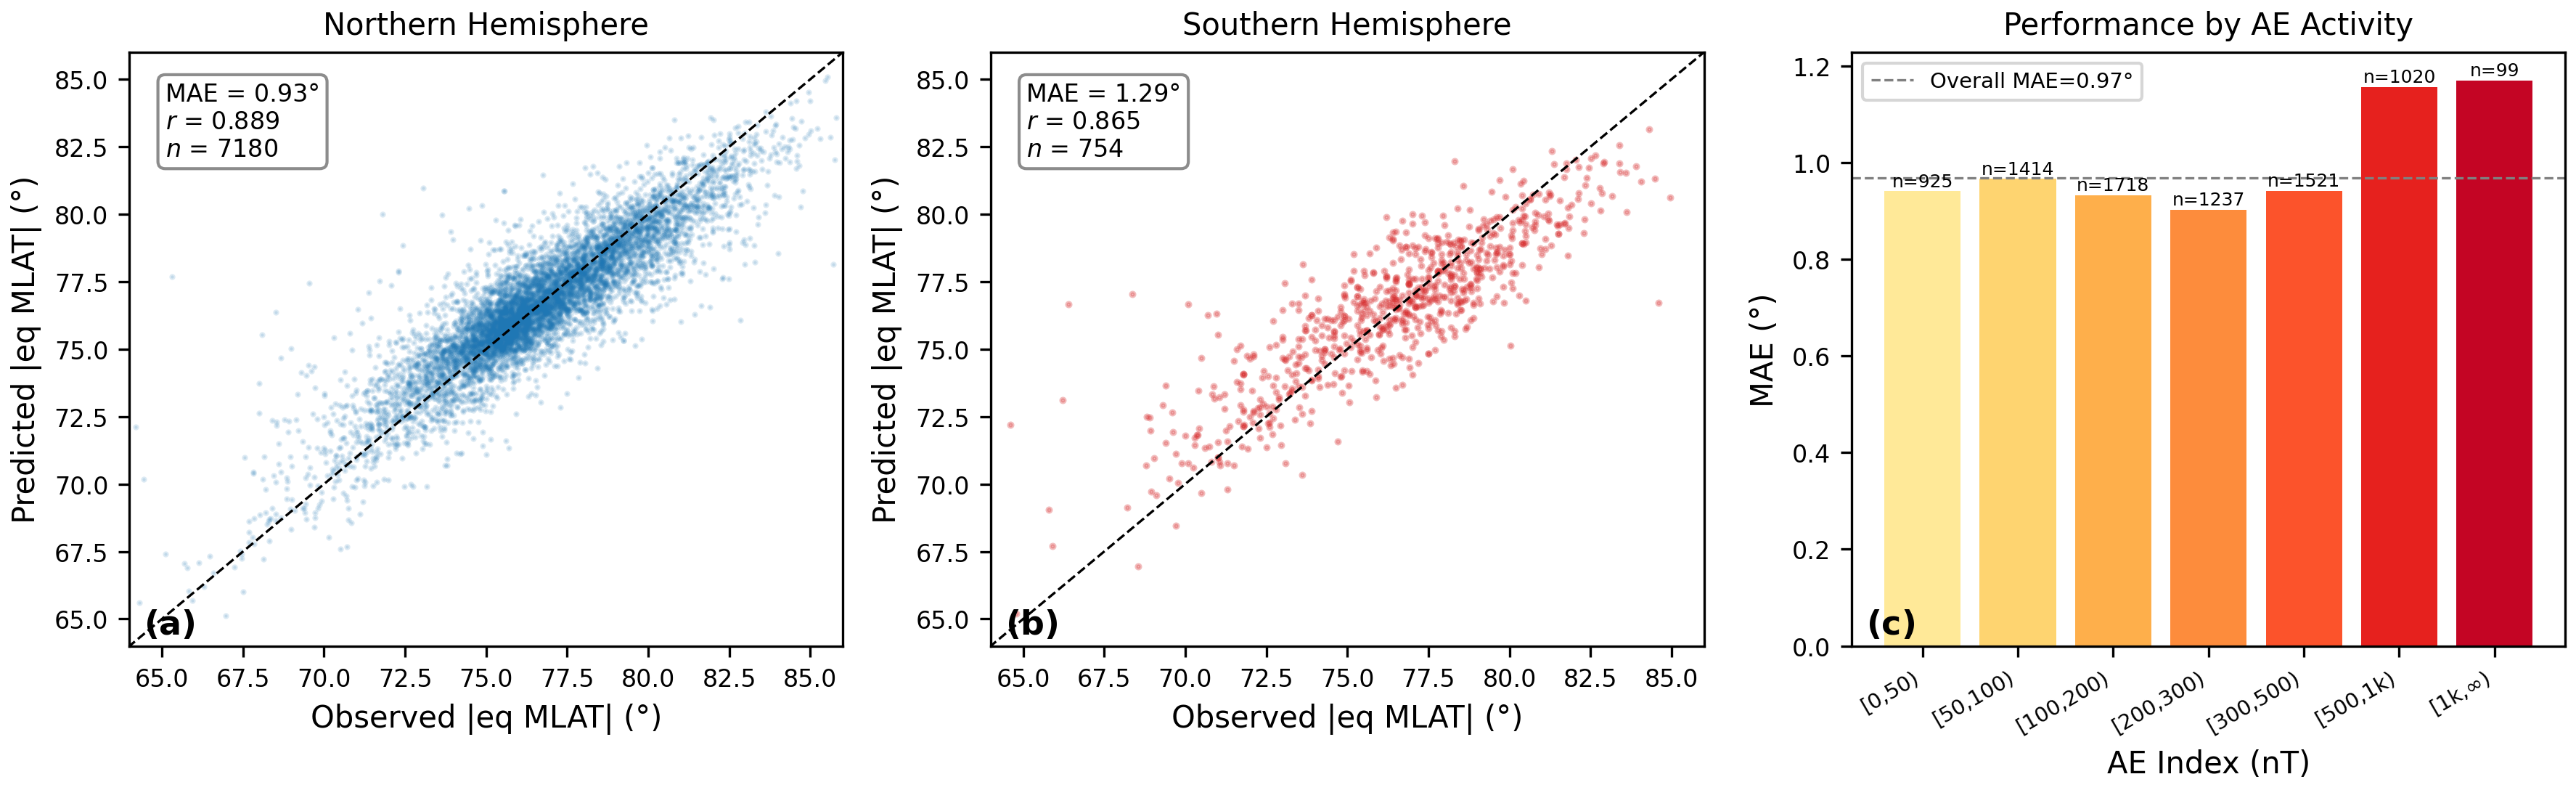
\includegraphics[width=\textwidth]{figures/fig10_hemi_ae.png}
\caption{Model performance stratified by hemisphere and geomagnetic activity. (a)--(b) Observed versus predicted equatorward MLAT for Northern and Southern Hemisphere crossings, respectively. (c) MAE by AE activity bin with sample counts annotated.}
\label{fig:hemi_ae}
\end{figure}

\textbf{Dipole tilt dependence.} To assess whether model performance is uniform across tilt conditions, we divide the test set into six tilt bins and compute MAE within each. The MAE ranges from 0.87\textdegree{} in the $[-35, -20)$\textdegree{} bin to 1.15\textdegree{} in the $[20, 35)$\textdegree{} bin. The elevated MAE at large positive tilt (summer Northern Hemisphere, $n = 467$) may reflect sampling imbalance or genuine physical complexity at extreme tilt angles. Overall, the model performs comparably across the full tilt range.

\textbf{Temporal generalization.} With 27~years of multi-satellite data, the model could in principle memorize satellite- or epoch-specific patterns. Leave-one-year-out (LOYO) cross-validation yields a mean MAE of $1.26 \pm 0.19$\textdegree{} across 23 held-out years ($n \geq 100$), with the worst individual year (1992) reaching MAE $\approx 1.7$\textdegree. A temporal split (train on pre-2008, test on 2008--2014) gives MAE = 1.11\textdegree, only 14\% higher than the random-split MAE. Both tests confirm that the model captures genuine solar wind--cusp relationships that generalize across solar cycles.

\textbf{Label uncertainty and irreducible error.} To estimate crossing-to-crossing variability in the cusp boundary labels, we identify 9{,}679 multi-crossing groups (same calendar day, same 0.5-hr MLT bin). The within-group standard deviation of $|$eq MLAT$|$ is $1.03 \pm 1.01$\textdegree, and the mean range is 2.35\textdegree. This spread represents an upper bound on combined observational and geophysical variability, including real cusp variability on sub-hour timescales and satellite orbit-path differences. The fact that the model MAE of 0.97\textdegree{} (or 1.11\textdegree{} under temporal holdout) is comparable to this within-group spread suggests that much of the remaining error is geophysical variability that no upstream solar wind model can predict.

% ======================================================================
\section{Discussion}
\label{sec:discussion}
% ======================================================================

\subsection{Physical Interpretation of the 60-Minute Timescale}

The dominant role of the 60-minute mean Newell coupling function in our model has a clear physical interpretation. Dayside magnetic reconnection opens magnetic flux, which is subsequently transported into the magnetotail. The cusp latitude reflects the total amount of open flux on the dayside, which is determined by the balance between the rate of flux opening (reconnection) and flux closure (nightside reconnection). This balance evolves on a timescale governed by the magnetospheric convection cycle, which \citet{burton1975dst} estimated at approximately 60 minutes.

\citet{newell2006cusp} independently found that their coupling function correlations were optimized with a 60$\pm$5 minute averaging window, attributing this to the time required for the magnetosphere to reconfigure in response to changed IMF conditions. \citet{lockwood2019coupling} further demonstrated that transpolar voltage---closely related to cusp latitude---responds to the time-integrated reconnection rate with a similar characteristic timescale.

Our feature importance analysis is consistent with this picture: the 60-minute features consistently outperform shorter timescales (Figure~\ref{fig:timescale}), and the 60-minute mean coupling function has the highest gain-based importance ($\sim$31\%) and the largest mean absolute SHAP value (1.07\textdegree). The gain ranking, the SHAP analysis, and the timescale ablation (Section~\ref{sec:results}) all point to the same window. None of these three methods---gain, SHAP, PDP---can establish causation when predictors are correlated. They do, however, point consistently at the same timescale, and that timescale matches prior reconnection-cycle estimates.

\subsection{Why XGBoost Outperforms Linear Models}

The 46\% MAE reduction achieved by XGBoost over the best linear coupling function can be decomposed via the baseline ladder. Ridge regression on the same 74-feature input set (MAE = 1.41\textdegree) attributes 22\% of the reduction to feature richness alone. GBR-300 (standard gradient boosting, MAE = 1.11\textdegree) adds a further 21\% by capturing nonlinear relationships. XGBoost-1000 (MAE = 0.97\textdegree) adds a final 13\% through deeper trees and extended boosting rounds. Taken together, nonlinear modeling (21\%~+~13\% = 34\%) accounts for the larger share of the total improvement relative to the single-parameter linear baseline.

\textbf{Nonlinear dependences.} \citet{newell2006cusp} showed that cusp latitude depends on $E_{WAV}^{2/3}$, not linearly on $E_{WAV}$. Our partial dependence plots (Figure~\ref{fig:partial_dep}b) confirm this nonlinear dependence, which XGBoost captures automatically through recursive tree splitting without requiring the functional form to be specified \textit{a priori}.

\textbf{Multi-parameter interactions.} Linear models based on a single coupling function cannot capture interactions between parameters. The cusp latitude depends simultaneously on IMF direction, solar wind dynamic pressure \cite{shue1997magnetopause, shue1998magnetopause}, dipole tilt \cite{newell1989tilt}, and IMF $B_y$ \cite{anderson2024cusp, cowley1981imfby}. XGBoost naturally captures these interactions through conditional tree branching.

\textbf{Historical context.} Linear models typically use instantaneous or single-window-averaged solar wind measurements. Our 74-feature set provides the model with information about how the solar wind has evolved over the preceding hour at multiple timescales, enabling it to infer the magnetospheric state more completely than any single snapshot can provide.

\citet{lockwood2022pitfalls} warned about overfitting in coupling function studies. Our model is evaluated on data never seen during training, and the feature importance hierarchy (coupling functions $>$ IMF $>$ tilt $>$ pressure) is physically sensible. Five-fold CV stability (MAE = $0.96 \pm 0.01$\textdegree) further supports generalization.

\subsection{Operational Potential and Limitations}

All 74 input features used by our model are derivable from the OMNI dataset or from upstream solar wind monitors such as DSCOVR at the L1 Lagrange point \cite{king2005omni}, so the solar wind alone carries enough information to predict along-track cusp boundary latitude. Table~\ref{tab:computational} compares the computational characteristics of the models evaluated in this study. In batch mode, XGBoost inference requires $\sim$0.04~ms per sample ($\sim$0.3~s for the full test set), and training completes in $\sim$80~s on 8 CPU cores, so the model can be retrained quickly when new data become available.

Operational deployment faces practical caveats. Real-time L1 data contain gaps; our model requires complete 60-minute windows and would need a gap-filling strategy. The model was trained on OMNI-propagated data, so performance on raw L1 measurements is unvalidated. The LOYO MAE ($1.26 \pm 0.19$\textdegree) and temporal-holdout MAE (1.11\textdegree) are more realistic operational estimates than the random-split MAE. The model predicts the cusp at a single MLT, not a 2-D map. Real-time validation with L1 data streams and gap-handling would be needed before deployment.

\begin{table}[htbp]
\centering
\caption{Computational comparison of model architectures. Tree-based and linear model training times are for the full 39,668-sample dataset; neural network training times are from architecture search on the $\sim$11,700-sample subset. Inference times are per-sample estimates.}
\label{tab:computational}
\begin{tabular}{lccc}
\toprule
Model & Parameters & Training Time & Inference \\
\midrule
Linear regression (1 feature) & 1 & $<0.1$~s (CPU) & $<0.1$~ms \\
Ridge regression (74 features) & 74 & $<0.1$~s (CPU) & $<0.1$~ms \\
GBR-300 (depth 5) & $\sim$300K leaf nodes & $\sim$90~s (CPU) & 0.1~ms (batch) \\
XGBoost-1000 & $\sim$1M leaf nodes & $\sim$80~s (8 CPU) & 0.04~ms (batch) \\
MLP-gelu & 20,068 & $\sim$11~s (NVIDIA V100 GPU) & $\sim$2~ms \\
ResMLP-4blk-128 & 142,468 & $\sim$36~s (NVIDIA V100 GPU) & $\sim$5~ms \\
TabTransformer-d128-L2 & 416,260 & $\sim$136~s (NVIDIA V100 GPU) & $\sim$10~ms \\
\bottomrule
\end{tabular}
\end{table}

Several limitations should be noted. (1)~OMNI propagation uncertainty, especially in $B_z$ which has the shortest spatial coherence scale \cite{king2005omni}, affects all solar-wind-based models. (2)~Extreme geomagnetic storms are rare in the 1987--2014 training set, so performance may degrade in those regimes. (3)~The residual $\sim$1\textdegree{} error likely combines OMNI measurement noise ($\sim$0.48~nT random $B_z$ difference between spacecraft; \citealt{king2005omni}), 5--10~minute propagation timing ambiguity, and magnetospheric dynamics (substorms, FTEs) not predictable from upstream data \cite{pitout2021cluster}. (4)~Extreme dipole tilt angles are under-represented; the elevated MAE at large positive tilt (1.15\textdegree) may partly reflect this imbalance.

\subsection{MLT Prediction and Comparison With Other Models}

The lower $R^2$ for MLT ($\sim$0.48--0.50) than MLAT ($\sim$0.79) largely reflects the narrow intrinsic spread of cusp MLT ($\sigma \approx 1$~hr around noon; \citealt{newell1988cusp}). An MAE of 0.73--0.77~hr still pins the cusp to within about half an hour. The cusp's MLT concentration is tight enough ($\sim$1100--1300~MLT) that a linear treatment is adequate; a wrapped-normal model would be needed only for a broader circular distribution. The main MLT driver is IMF $B_y$ \cite{cowley1981imfby, anderson2024cusp}, which shifts the cusp dawn-duskward by typically $< 1$~hr.

Among recent ML applications to magnetospheric boundaries, \citet{feng2025auroral} used XGBoost for auroral oval prediction from Kp alone (3-hour resolution), while \citet{aghabozorgi2024magnetopause} predicted magnetopause standoff distance from solar wind data with similar OMNI propagation limitations. XGBoost's advantage over neural networks on our 74-feature tabular input agrees with the broader finding of \citet{grinsztajn2022tree} that tree-based models excel on heterogeneous tabular data.

% ======================================================================
\section{Summary and Conclusions}
\label{sec:conclusions}
% ======================================================================

We have presented the first machine learning model for predicting ionospheric cusp boundary locations from solar wind parameters. Our main findings are:

\begin{enumerate}
\item \textbf{Improved accuracy:} Equatorward cusp MLAT MAE = 1.11\textdegree{} (temporal holdout), $1.26 \pm 0.19$\textdegree{} (LOYO), 0.97\textdegree{} (random split, $r = 0.887$)---a 40--46\% reduction over the Newell baseline (1.80\textdegree; \citealt{newell2006cusp}). Poleward MLAT, equatorward MLT, and mean MLT achieve 0.95\textdegree, 0.77~hr, and 0.73~hr.

\item \textbf{60-minute timescale dominance:} The 60-minute mean Newell coupling function accounts for $\sim$31\% of gain-based feature importance; SHAP analysis confirms it as the dominant predictor (mean $|\text{SHAP}| = 1.07$\textdegree). The 60-minute history features consistently outperform 15- and 30-minute windows, consistent with the interpretation that cusp latitude responds to approximately one hour of integrated dayside reconnection.

\item \textbf{Physical consistency:} Partial dependence analysis recovers the dipole tilt slope of $\sim$0.05\textdegree/\textdegree{} \cite{newell1989tilt}, the nonlinear coupling function dependence \cite{newell2006cusp}, and the dynamic pressure effect \cite{shue1997magnetopause}, which agrees with earlier results from direct physical analysis.

\item \textbf{Accuracy relative to cusp scale:} The model temporal-holdout MAE of 1.11\textdegree{} is smaller than the full cusp extent ($\sim$3--4\textdegree{} MLAT; \citealp{zhang2013lfm}). On random splits, 63\% of predictions fall within 1\textdegree{} and 89\% within 2\textdegree{}. Multi-crossing overlap analysis yields a crossing-to-crossing spread of $\sim$1\textdegree{}, an upper bound on combined geophysical variability. Remaining errors likely reflect this variability, OMNI measurement uncertainties, propagation timing, and internal magnetospheric dynamics.

\item \textbf{Tree model superiority:} XGBoost-1000 (MAE = 0.97\textdegree{}) substantially outperforms all tested neural network architectures (MLP, ResMLP, TabTransformer; best: 1.02\textdegree{}) and conventional GBR-300 (1.11\textdegree{}) on this tabular prediction problem, consistent with the advantage of tuned gradient-boosted trees for structured data \citep{grinsztajn2022tree}. Note that NN and GBR comparisons involve different evaluation subsets; the ranking is consistent but the gap sizes should be interpreted with caution.

\item \textbf{Solar wind predictability:} All 74 inputs are derivable from upstream solar wind monitors, so the solar wind alone provides enough information to predict along-track cusp boundary position with sub-degree precision. Full operational deployment would require validation with real-time L1 data, reliable gap-handling for 60-minute history windows, and extension to the two-dimensional cusp structure.
\end{enumerate}

Natural extensions include solar-cycle cross-validation, focused evaluation on extreme storms, and expansion to 2-D cusp maps using multi-satellite constellations. The trained model and database will be released through Zenodo on acceptance.

\section*{Conflict of Interest}
The authors declare no conflicts of interest relevant to this study.

\section*{Data Availability Statement}
The DMSP SSJ/4 and SSJ/5 particle precipitation data are publicly available from the NOAA National Centers for Environmental Information (NCEI; \url{https://www.ncei.noaa.gov/data/dmsp-space-weather-sensors/}). The OMNI solar wind and IMF data were obtained from the NASA Goddard Space Flight Center OMNIWeb interface (\url{https://omniweb.gsfc.nasa.gov}; \citealt{king2005omni}). The cusp crossing database (48,056 events, 1987--2014) and trained XGBoost model weights are archived at Zenodo (\url{https://doi.org/10.5281/zenodo.19340793}). Analysis code is available at \url{https://github.com/YiwenZhu77/cuspML}.

\section*{Acknowledgments}
The DMSP SSJ/4 and SSJ/5 data were obtained from the NCEI. The OMNI data were obtained from the NASA Goddard Space Flight Center OMNIWeb interface. This work is supported by NASA DRIVE Science Center for Geospace Storms Grant 80NSSC22M0163. We also acknowledge the use of computational resources at the National Center for Atmospheric Research (NCAR)-Wyoming Supercomputing Center provided by the National Science Foundation and the State of Wyoming, and supported by NCAR's Computational and Information Systems Laboratory.

\bibliography{references}

\end{document}
